\documentclass[aspectratio=169,11pt]{beamer}

\usepackage[T1]{fontenc}
\usepackage[utf8]{inputenc}
\usepackage{graphicx}
\usepackage{booktabs}
\usepackage{tabularx}
\usepackage{array}
\usepackage{multirow}
\usepackage{amsmath}
\usepackage{adjustbox}
\usepackage{ragged2e}
\usepackage{tikz}
\usetikzlibrary{arrows.meta, positioning, shapes.geometric, fit, calc}

\usetheme{Madrid}
\setbeamertemplate{navigation symbols}{}
\setbeamertemplate{footline}[frame number]

\definecolor{ThesisBlue}{HTML}{113A5C}
\definecolor{ThesisGold}{HTML}{C78B2B}
\definecolor{ThesisInk}{HTML}{21313F}
\definecolor{ThesisSoft}{HTML}{EEF3F7}
\definecolor{ThesisAccent}{HTML}{DCE8F2}

\setbeamercolor{structure}{fg=ThesisBlue}
\setbeamercolor{title}{fg=white,bg=ThesisBlue}
\setbeamercolor{frametitle}{fg=white,bg=ThesisBlue}
\setbeamercolor{section in toc}{fg=ThesisBlue}
\setbeamercolor{block title}{fg=white,bg=ThesisBlue}
\setbeamercolor{block body}{fg=black,bg=ThesisSoft}
\setbeamercolor{alerted text}{fg=ThesisGold}
\setbeamercolor{itemize item}{fg=ThesisBlue}
\setbeamercolor{itemize subitem}{fg=ThesisBlue}

\setbeamertemplate{blocks}[rounded][shadow=false]
\setbeamertemplate{itemize item}{\color{ThesisGold}$\blacktriangleright$}
\setbeamertemplate{itemize subitem}{\color{ThesisGold}$\triangleright$}
\setbeamersize{text margin left=6mm,text margin right=6mm}

\newenvironment{tightitemize}{
  \begin{itemize}
    \setlength{\itemsep}{2pt}
    \setlength{\parskip}{0pt}
}{\end{itemize}}

\newcommand{\highlight}[1]{\textcolor{ThesisBlue}{\textbf{#1}}}
\newcommand{\metric}[1]{\textbf{\textcolor{ThesisBlue}{#1}}}
\newcommand{\best}[1]{{\color{black}\textbf{#1}}}
\newcommand{\runnerup}[1]{{\color{black}\textbf{#1}}}

\title{From Legal Text to Legal Graphs}
\subtitle{A Detailed Thesis Presentation on Leakage-Safe Legal Judgment Prediction with Heterogeneous Graph Neural Networks}
\author{Ziv Barretto}
\institute{Thesis Presentation}
\date{April 2026}

\begin{document}

\begin{frame}[plain]
  \titlepage
\end{frame}

\begin{frame}{Roadmap}
  \tableofcontents
\end{frame}

\section{Motivation and Research Questions}

\begin{frame}{Why This Problem Matters}
  \begin{columns}[T]
    \begin{column}{0.58\textwidth}
      \begin{tightitemize}
        \item \highlight{Access to justice} in India is constrained by large judicial backlogs, long litigation cycles, and uneven access to legal assistance.
        \item The thesis does \highlight{not} argue for automating judges. It argues for \highlight{decision support}: tools that organize case material, surface patterns, and assist legal research.
        \item Legal Judgment Prediction (LJP) is valuable only if it predicts from \highlight{pre-decision signals} such as facts, arguments, statutes, and precedents.
        \item If a model can read phrases like ``appeal allowed'' or memorize judges, the task collapses into \highlight{answer recovery}, not legal reasoning.
      \end{tightitemize}
    \end{column}
    \begin{column}{0.38\textwidth}
      \begin{block}{Thesis Position}
        A credible legal prediction system must be:
        \begin{tightitemize}
          \item structurally faithful,
          \item leakage-safe,
          \item interpretable,
          \item and able to transfer beyond one narrow legal niche.
        \end{tightitemize}
      \end{block}
    \end{column}
  \end{columns}
\end{frame}

\begin{frame}{What Exactly Is Being Predicted?}
  \small
  \begin{columns}[T]
    \begin{column}{0.55\textwidth}
      \begin{block}{Target Definition}
        Outcome prediction from the \highlight{appellant/petitioner perspective}:
        \begin{tightitemize}
          \item \texttt{appellant\_won} $(+1)$
          \item \texttt{appellant\_lost} $(-1)$
          \item \texttt{postponed\_or\_procedural} $(0)$
        \end{tightitemize}
      \end{block}
      \begin{block}{Prediction Task Used for the Main Model}
        The main GNN experiments use the \highlight{binary subset}:
        \begin{tightitemize}
          \item win vs.\ loss only
          \item procedural/neutral cases excluded from training
          \item outcome-bearing text removed before graph construction
        \end{tightitemize}
      \end{block}
    \end{column}
    \begin{column}{0.41\textwidth}
      \begin{block}{Why This Definition Matters}
        \begin{tightitemize}
          \item prevents trivial leakage from operative text,
          \item makes the task experimentally honest,
          \item forces the model to work from pre-decision evidence,
          \item aligns evaluation with realistic case-support use.
        \end{tightitemize}
      \end{block}
    \end{column}
  \end{columns}
\end{frame}

\begin{frame}{Why Ordinary Document Classification Is Not Enough}
  \small
  \begin{columns}[T]
    \begin{column}{0.50\textwidth}
      \begin{tightitemize}
        \item Judgments mix \highlight{facts, procedural history, party arguments, precedent citations, and reasoning} in one long document.
        \item Indian judgments are noisy: OCR errors, citation variation, transliterated names, multilingual fragments, inconsistent formatting.
        \item One legal matter may produce \highlight{multiple hearing-stage documents}; treating each PDF as a separate case corrupts the representation and the label.
        \item The core legal signal is \highlight{relational}: facts connect to arguments, arguments cite statutes, provisions belong to statutes, cases cite precedents.
      \end{tightitemize}
    \end{column}
    \begin{column}{0.46\textwidth}
      \centering
      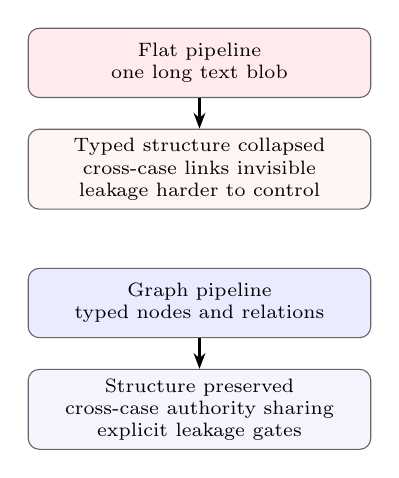
\begin{tikzpicture}[
        every node/.style={font=\scriptsize},
        box/.style={draw=black!60, rounded corners, align=center, minimum width=4.35cm, minimum height=0.88cm},
        arrow/.style={-{Stealth[length=2mm]}, thick}
      ]
        \node[box, fill=red!8] (flat) at (0,1.35) {Flat pipeline\\one long text blob};
        \node[box, fill=red!4] (loss) at (0,0) {Typed structure collapsed\\cross-case links invisible\\leakage harder to control};
        \node[box, fill=blue!8] (graph) at (0,-1.70) {Graph pipeline\\typed nodes and relations};
        \node[box, fill=blue!4] (gain) at (0,-3.05) {Structure preserved\\cross-case authority sharing\\explicit leakage gates};
        \draw[arrow] (flat) -- (loss);
        \draw[arrow] (graph) -- (gain);
      \end{tikzpicture}
    \end{column}
  \end{columns}
\end{frame}

\begin{frame}{Research Questions and Thesis Claims}
  \scriptsize
  \begin{block}{Research Questions}
    \begin{tightitemize}
      \item \highlight{RQ1}: Can Indian court judgments be converted into a legally coherent and leakage-safe structured corpus at scale?
      \item \highlight{RQ2}: Does a heterogeneous graph representation improve outcome prediction over a no-graph embedding baseline and graph ablations?
      \item \highlight{RQ3}: Which parts of the graph actually carry the predictive signal?
      \item \highlight{RQ4}: Can individual predictions be explained in legally named terms, and does the learned representation transfer to an unseen legal domain?
    \end{tightitemize}
  \end{block}
  \begin{block}{Claims This Thesis Defends}
    \begin{tightitemize}
      \item A reasoning-focused heterogeneous graph is a better fit than flat document classification.
      \item Leakage can be constrained through schema design, field filtering, rhetorical-role filtering, phrase masking, and temporal gating.
      \item The learned signal is primarily legal-text structure plus shared authority nodes, not identity shortcuts.
      \item The model is interpretable at both the global and case level.
    \end{tightitemize}
  \end{block}
\end{frame}

\section{Pipeline and Data Construction}

\begin{frame}{End-to-End Pipeline}
  \centering
  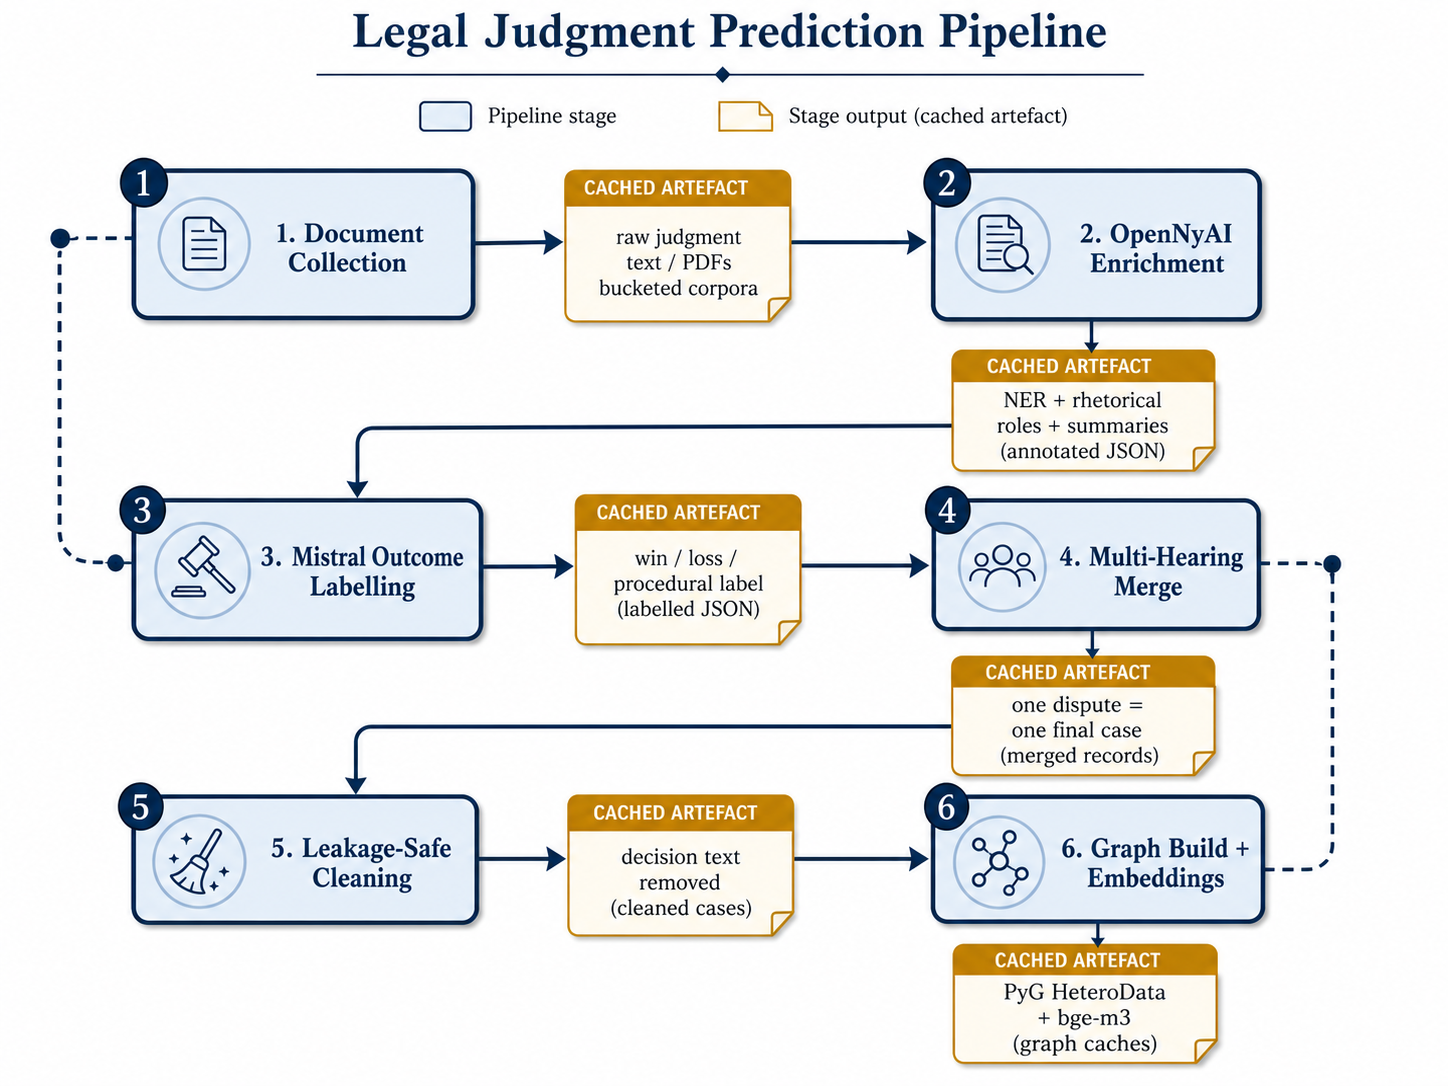
\includegraphics[width=0.96\linewidth,height=0.72\textheight,keepaspectratio]{new_slide_figures/304f1a23-9c64-4124-a367-0ce90b30dd5b.png}

  \vspace{0.3em}
  \small
  Each pipeline stage produces a cached artefact that feeds the next stage, so every step is independently re-runnable and auditable.
\end{frame}

\begin{frame}{Corpus Design and Legal Domains}
  \scriptsize
  \begin{columns}[T]
    \begin{column}{0.42\textwidth}
      \begin{block}{Collection Strategy and Domain Split}
        \begin{tightitemize}
          \item Source: Indian Kanoon
          \item Crawl by \highlight{court-month windows} to avoid result truncation
          \item Bucket locally by regex/statutory rules instead of relying on search-engine bias
          \item Aim: comparable domain scale for fair cross-domain evaluation
          \item Domains: Family \& Matrimonial, Financial Fraud, Land \& Property, Motor Accidents, Sexual Offences
        \end{tightitemize}
      \end{block}
    \end{column}
    \begin{column}{0.54\textwidth}
      \centering
      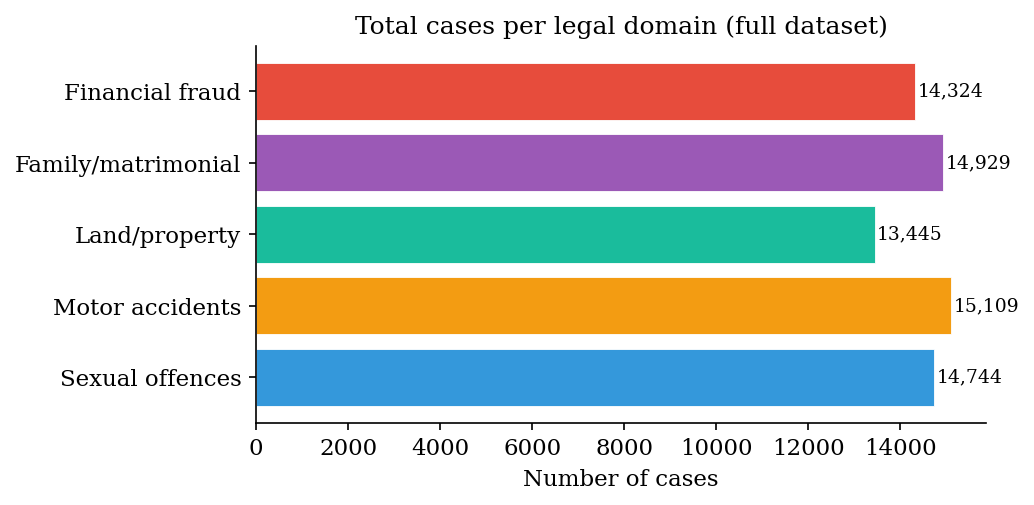
\includegraphics[width=\linewidth,height=0.52\textheight,keepaspectratio]{figures/01_case_counts_full.png}

      \vspace{0.3em}
      \scriptsize
      After multi-hearing merging, the domains remain closely balanced in size, which makes pooled evaluation and per-domain comparison meaningful.
    \end{column}
  \end{columns}
\end{frame}

\begin{frame}{OpenNyAI Enrichment Stage}
  \scriptsize
  \begin{block}{What OpenNyAI Adds to Each Judgment}
    \begin{adjustbox}{max width=\textwidth}
      \begin{tabular}{p{2.4cm}p{4.0cm}p{5.0cm}}
        \toprule
        \textbf{Component} & \textbf{Output} & \textbf{Why It Matters} \\
        \midrule
        Legal NER & statutes, provisions, precedents, courts, judges, parties, lawyers, case numbers & supplies typed legal entities that can become graph nodes \\
        Rhetorical Role Classifier & sentence-level labels such as preamble, facts, arguments, RPC, RLC & separates usable pre-decision content from outcome-bearing text \\
        Summarizer & structured blocks for preamble, facts, arguments, decision & gives compact sections for outcome labelling and graph text nodes \\
        \bottomrule
      \end{tabular}
    \end{adjustbox}
  \end{block}
  \begin{block}{Why This Is a Good Fit for Indian Legal Text}
    \begin{tightitemize}
      \item It is trained on Indian legal discourse rather than generic text.
      \item It recognizes statutes, provisions, precedent citations, and party roles that generic NLP often misses.
      \item It produces the typed signals needed both for graph construction and for leakage-safe filtering.
    \end{tightitemize}
  \end{block}
\end{frame}

\begin{frame}{Multi-Hearing Consolidation}
  \scriptsize
  \begin{columns}[T]
    \begin{column}{0.46\textwidth}
      \begin{block}{Why Merging Is Necessary}
        One legal dispute may produce several hearing-stage documents. Without merging:
        \begin{tightitemize}
          \item the same dispute becomes multiple case nodes,
          \item the final label is not aligned to earlier hearings,
          \item shared entities get double-counted as fake independent evidence.
        \end{tightitemize}
      \end{block}
      \begin{block}{v3 Merge Rule}
        Merge only when both match:
        \begin{tightitemize}
          \item case title, and
          \item court registration number.
        \end{tightitemize}
        FIR number is explicitly \highlight{not} used, because one FIR can spawn different court proceedings.
      \end{block}
    \end{column}
    \begin{column}{0.50\textwidth}
      \scriptsize
      \begin{tabular}{lrr}
        \toprule
        Bucket & Inputs & Final Cases \\
        \midrule
        Family \& Matrimonial & 15{,}800 & 15{,}306 \\
        Financial Fraud & 15{,}014 & 14{,}615 \\
        Land \& Property & 14{,}324 & 14{,}051 \\
        Motor Accidents & 15{,}271 & 15{,}236 \\
        Sexual Offences & 15{,}532 & 14{,}596 \\
        \midrule
        Total & 75{,}941 & 73{,}804 \\
        \bottomrule
      \end{tabular}

      \vspace{0.8em}
      \begin{block}{Merge Outcome}
        \begin{tightitemize}
          \item 2{,}111 earlier hearing documents were folded into later final-case records.
          \item Sexual-offence matters merge most often; motor-accident cases least.
          \item Every merge is logged so the operation remains auditable.
        \end{tightitemize}
      \end{block}
    \end{column}
  \end{columns}
\end{frame}

\begin{frame}{Outcome Target and Class Balance}
  \scriptsize
  \begin{columns}[T]
    \begin{column}{0.42\textwidth}
      \begin{block}{Three Labels from the Appellant's Perspective}
        \begin{tightitemize}
          \item \texttt{won}: relief granted, appeal/petition allowed, conviction quashed, bail granted
          \item \texttt{lost}: appeal dismissed, relief denied, bail refused
          \item \texttt{procedural}: remand, adjournment, notice, no clear final outcome
        \end{tightitemize}
      \end{block}
      \small
      The pooled binary task is roughly \highlight{60\% win / 40\% loss}, so macro-F1 is reported alongside accuracy and ROC-AUC.
    \end{column}
    \begin{column}{0.54\textwidth}
      \centering
      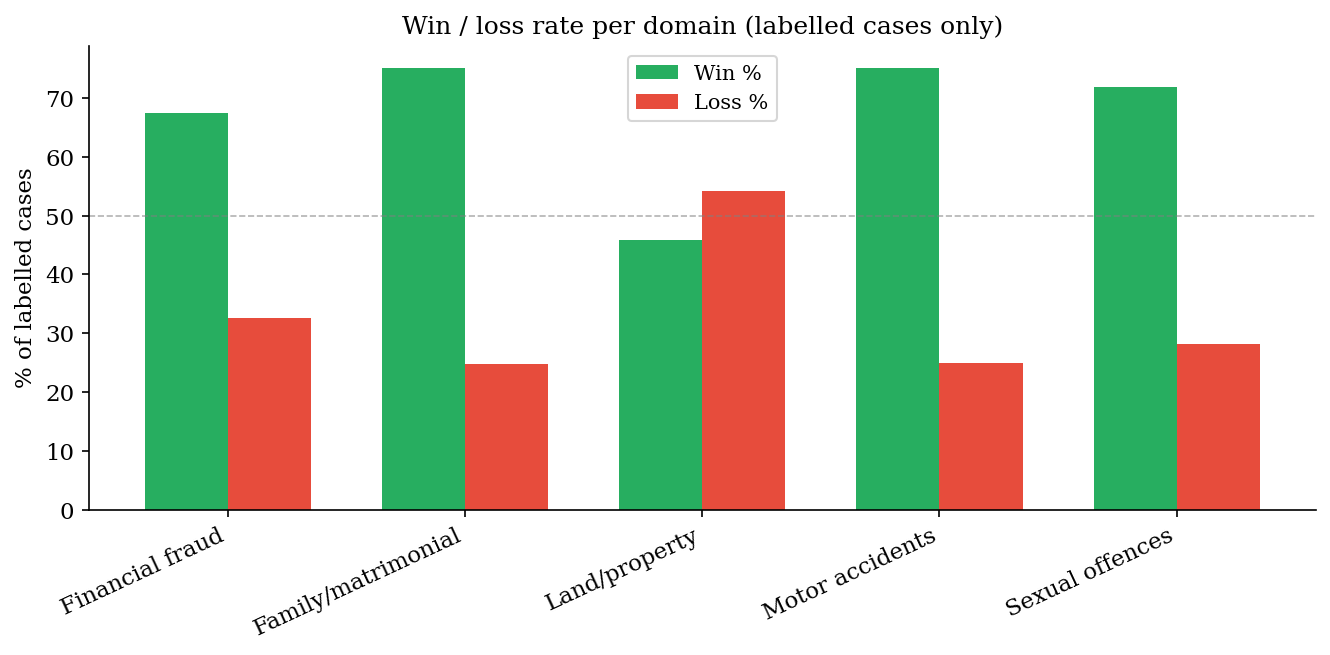
\includegraphics[width=\linewidth,height=0.52\textheight,keepaspectratio]{figures/03_outcome_rate_full.png}
    \end{column}
  \end{columns}
\end{frame}

\begin{frame}{Cross-Label Methodology}
  \tiny
  \begin{columns}[T,onlytextwidth]
    \begin{column}{0.55\textwidth}
      \begin{block}{Second Pass: Eight Binary Questions}
        \tiny
        \setlength{\tabcolsep}{3pt}
        \begin{tabular}{@{}p{1.25cm}p{0.45cm}p{4.85cm}@{}}
          \toprule
          Group & ID & Question labelled by Mistral \\
          \midrule
          Win & Q1 & Did the appellant win the case? \\
              & Q2 & Was the petition, appeal, or application allowed? \\
              & Q3 & Did the court rule in favour of the petitioner or appellant? \\
          Loss & Q4 & Did the respondent win the case? \\
               & Q5 & Was the petition, appeal, or application dismissed? \\
               & Q6 & Did the court rule against the appellant? \\
          Neutral & Q7 & Was the case adjourned, remanded, or deferred without a final decision? \\
                  & Q8 & Is there no clear final judgment in this case? \\
          \bottomrule
        \end{tabular}
      \end{block}
    \end{column}
    \begin{column}{0.41\textwidth}
      \begin{block}{Deterministic Final Label}
        The model returns JSON keys \texttt{q1}--\texttt{q8}, each 1 for yes or 0 for no.
        \[
          \begin{aligned}
            S_w&=q_1+q_2+q_3\\
            S_l&=q_4+q_5+q_6\\
            S_n&=q_7+q_8
          \end{aligned}
        \]
        \begin{tightitemize}
          \item If $S_n>0$: \texttt{procedural}.
          \item If both win and loss fire: majority wins; tie becomes \texttt{procedural}.
          \item If only win fires: \texttt{appellant\_won}.
          \item If only loss fires: \texttt{appellant\_lost}.
          \item If all answers are zero: \texttt{unknown} and excluded.
        \end{tightitemize}
      \end{block}
      \vspace{0.1em}
      \tiny
      This removes free-form label variance: the LLM only answers binary checks, and the final class is computed by rule.
    \end{column}
  \end{columns}
\end{frame}

\begin{frame}{Label Quality and Coverage}
  \scriptsize
  \begin{columns}[T,onlytextwidth]
    \begin{column}{0.50\textwidth}
      \centering
      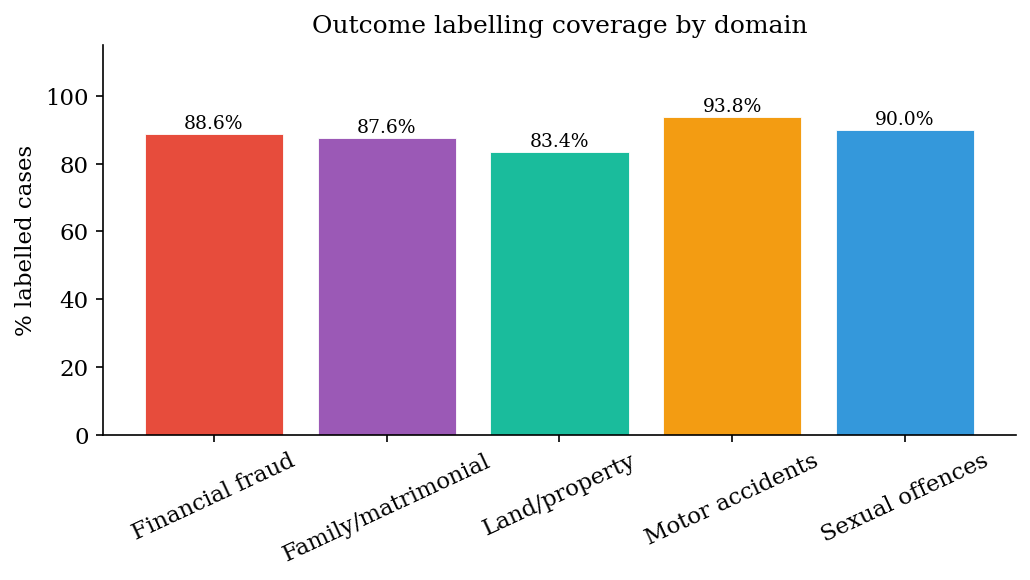
\includegraphics[width=\linewidth,height=0.55\textheight,keepaspectratio]{figures/08_labelling_coverage_full.png}

      \vspace{0.2em}
      \scriptsize
      Coverage is near-complete in every domain; malformed or ambiguous cases are excluded instead of force-labelled.
    \end{column}
    \begin{column}{0.46\textwidth}
      \begin{block}{Cross-Run Reliability Check}
        A second labelling pass using a different prompt design agreed with the first pass on \highlight{84.4\%} of 72{,}795 comparable files.
      \end{block}
      \scriptsize
      \begin{tabular}{lrr}
        \toprule
        Bucket & Files & Agreement \\
        \midrule
        Family \& Matrimonial & 15{,}017 & 86.9\% \\
        Financial Fraud & 14{,}342 & 83.8\% \\
        Land \& Property & 13{,}512 & 71.4\% \\
        Motor Accidents & 15{,}117 & 89.6\% \\
        Sexual Offences & 14{,}807 & 88.8\% \\
        \midrule
        Total & 72{,}795 & 84.4\% \\
        \bottomrule
      \end{tabular}

      \vspace{0.3em}
      \scriptsize
      The main disagreement is procedural vs.\ loss, not clean win vs.\ loss. That is why the primary prediction task excludes procedural cases.
    \end{column}
  \end{columns}
\end{frame}

\section{Graph Construction and Leakage Safety}

\begin{frame}{Why a Heterogeneous Graph?}
  \begin{columns}[T]
    \begin{column}{0.53\textwidth}
      \begin{tightitemize}
        \item A case is not just text. It is a \highlight{structured legal object} containing parties, courts, statutes, provisions, precedents, and argument blocks.
        \item Different node types play different legal roles. A court is not a statute; a petitioner is not a precedent.
        \item A graph preserves \highlight{within-case structure} and also \highlight{cross-case sharing} through legal authorities cited by many cases.
        \item This lets the model aggregate both:
        \begin{tightitemize}
          \item local evidence inside one case, and
          \item relational evidence across similar cases.
        \end{tightitemize}
      \end{tightitemize}
    \end{column}
    \begin{column}{0.43\textwidth}
      \begin{block}{Design Principle}
        Share only what is legally meaningful to share across cases:
        \begin{tightitemize}
          \item shared: statutes, provisions, precedents
          \item local: parties, lawyers, judges, courts
        \end{tightitemize}
        This keeps the graph useful \highlight{without turning identity into a shortcut}.
      \end{block}
    \end{column}
  \end{columns}
\end{frame}

\begin{frame}{Reasoning-Focused Graph Schema}
  \scriptsize
  \begin{columns}[T,onlytextwidth]
    \begin{column}{0.50\textwidth}
      \begin{block}{17 Node Types in Three Families}
        \begin{tightitemize}
          \item \highlight{Case}: one anchor node per dispute
          \item \highlight{Text nodes}: Preamble, Facts, Arguments, Petitioner Arguments, Respondent Arguments, Other Lawyer Arguments
          \item \highlight{Entity nodes}: Petitioner, Respondent, Petitioner Lawyer, Defence Lawyer, Lawyer, Court, Judge, Statute, Provision, Precedent
        \end{tightitemize}
      \end{block}
      \begin{block}{Deliberately Removed}
        \textsc{Org}, \textsc{GPE}, \textsc{Date}, and \textsc{Case\_Number} are excluded from the final reasoning-focused graph because they add noise and possible shortcuts.
      \end{block}
    \end{column}
    \begin{column}{0.44\textwidth}
      \tiny
      \begin{adjustbox}{max width=\linewidth}
        \begin{tabular}{p{2.8cm}p{3.0cm}p{3.2cm}}
          \toprule
          \textbf{Relation Family} & \textbf{Example Edge} & \textbf{Purpose} \\
          \midrule
          Case to text & \texttt{has\_facts} & attach textual evidence \\
          Case to entities & \texttt{heard\_in}, \texttt{has\_petitioner} & encode participants and forum \\
          Argument citations & \texttt{cites\_statute}, \texttt{cites\_precedent} & preserve legal reasoning context \\
          Provision hierarchy & \texttt{belongs\_to\_statute} & link sections to statutes \\
          Argument ownership & party/lawyer to argument blocks & keep side-specific discourse structure \\
          \bottomrule
        \end{tabular}
      \end{adjustbox}
    \end{column}
  \end{columns}
\end{frame}

\begin{frame}{Single-Case Graph Structure}
  \centering
  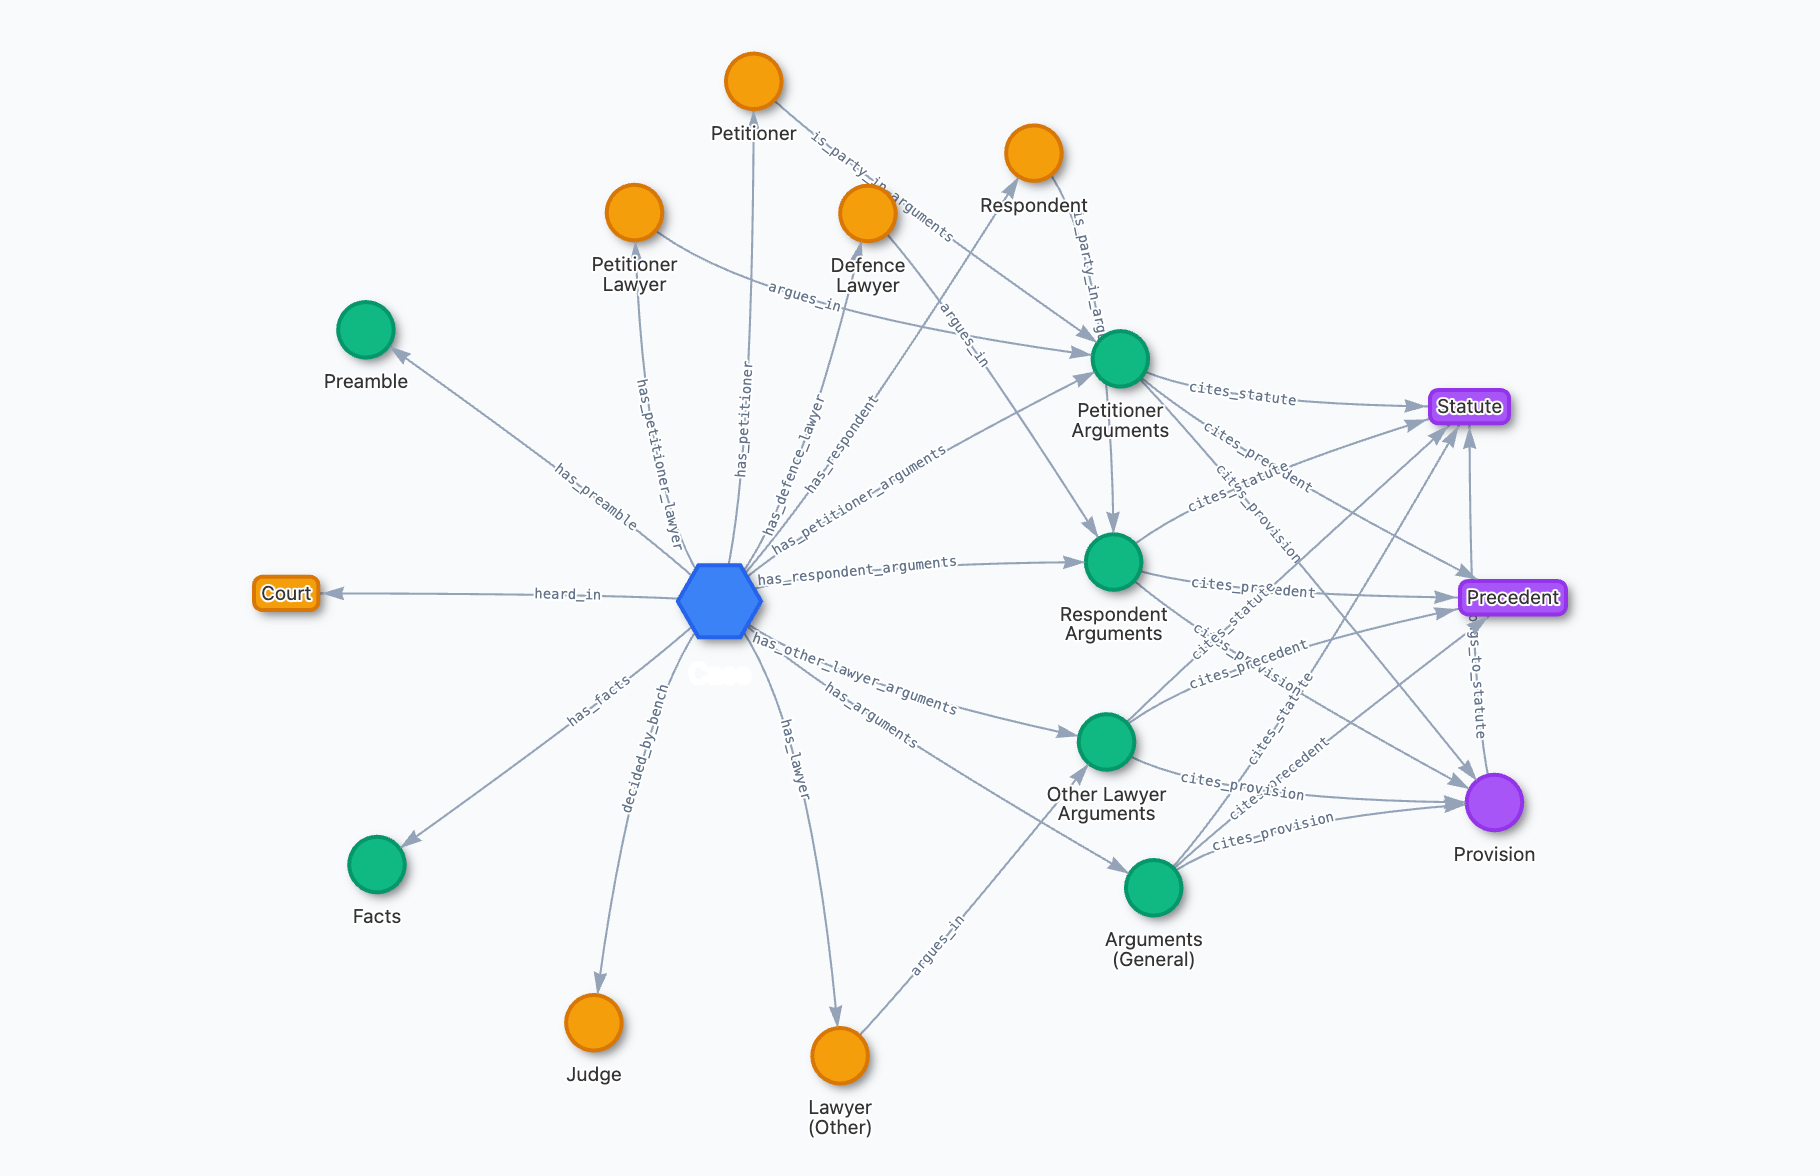
\includegraphics[width=0.96\linewidth,height=0.72\textheight,keepaspectratio]{new_slide_figures/legal_graph_ontology.png}

  \vspace{0.2em}
  \scriptsize
  Reasoning-focused ontology for the case graph: typed legal entities, text nodes, and authority links used by the heterogeneous graph.
\end{frame}

\begin{frame}{Cross-Case Sharing and Leakage Control}
  \centering
  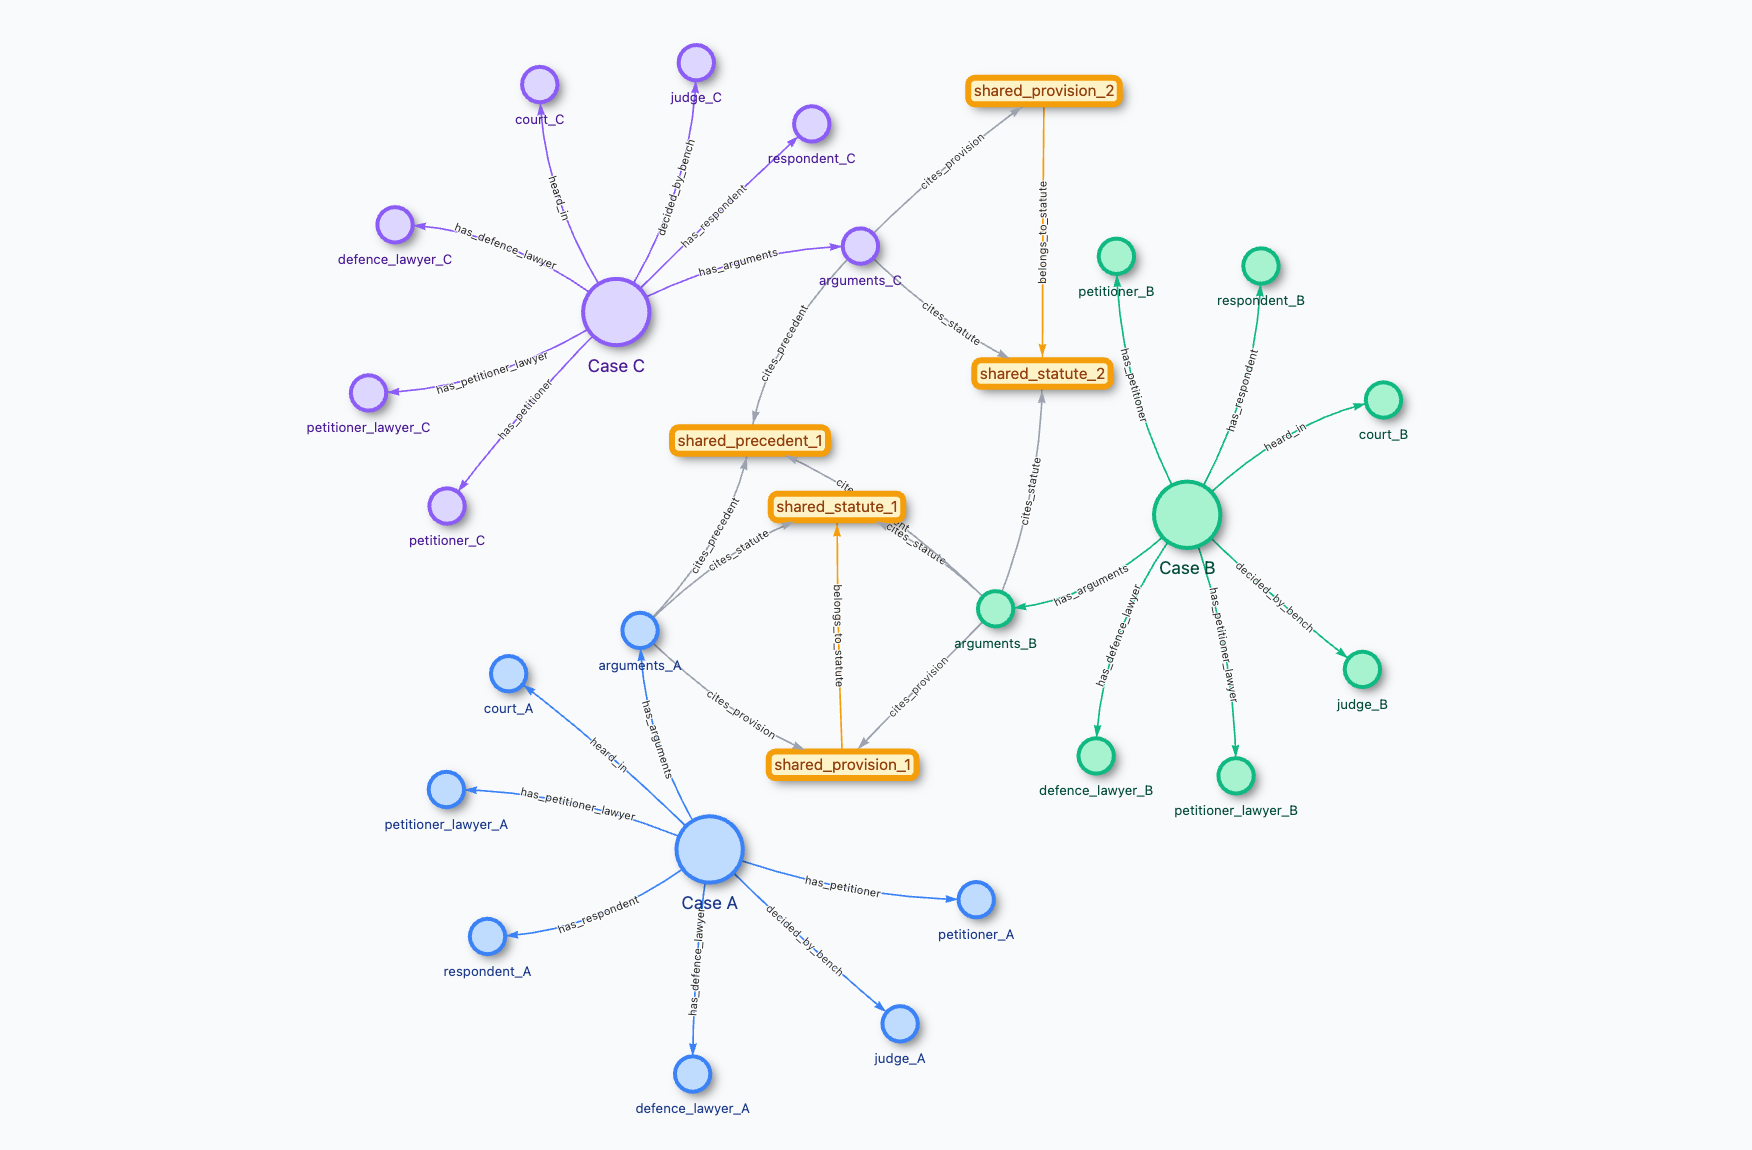
\includegraphics[width=0.96\linewidth,height=0.72\textheight,keepaspectratio]{new_slide_figures/cross_case_graph.png}

  \vspace{0.2em}
  \scriptsize
  Three case clusters keep identity local; only statutes, provisions, and precedents bridge across cases. Leakage gates govern what enters the graph at build time.
\end{frame}

\begin{frame}{Leakage Prevention Is a First-Class Design Constraint}
  \centering
  \resizebox{0.98\textwidth}{!}{%
  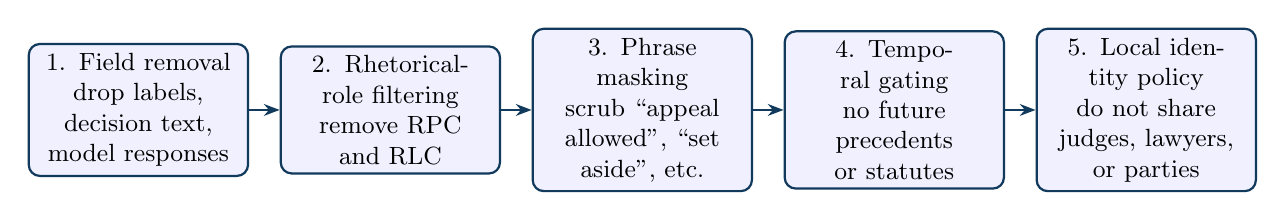
\begin{tikzpicture}[
    every node/.style={font=\small},
    gate/.style={rectangle, rounded corners, draw=ThesisBlue, thick, fill=blue!6, minimum width=2.75cm, minimum height=1.05cm, text width=2.55cm, align=center},
    arrow/.style={-{Stealth[length=2mm]}, thick, draw=ThesisBlue}
  ]
    \node[gate] (g1) at (0,0) {1. Field removal\\drop labels, decision text, model responses};
    \node[gate] (g2) at (3.2,0) {2. Rhetorical-role filtering\\remove RPC and RLC};
    \node[gate] (g3) at (6.4,0) {3. Phrase masking\\scrub ``appeal allowed'', ``set aside'', etc.};
    \node[gate] (g4) at (9.6,0) {4. Temporal gating\\no future precedents or statutes};
    \node[gate] (g5) at (12.8,0) {5. Local identity policy\\do not share judges, lawyers, or parties};
    \draw[arrow] (g1) -- (g2);
    \draw[arrow] (g2) -- (g3);
    \draw[arrow] (g3) -- (g4);
    \draw[arrow] (g4) -- (g5);
  \end{tikzpicture}}

  \vspace{0.9em}
  \begin{block}{Interpretation}
    The model is forced to see a \highlight{pre-decision representation of the dispute}: who the parties are, what happened, what each side argued, and what law they cited, but not the ruling itself.
  \end{block}
\end{frame}

\section{Graph Analysis and Structural Findings}

\begin{frame}{Hub Dominance and Heavy-Tailed Structure}
  \begin{columns}[T,onlytextwidth]
    \begin{column}{0.42\textwidth}
      \scriptsize
      \begin{adjustbox}{max width=\linewidth}
        \begin{tabular}{p{3.0cm}p{1.4cm}p{1.4cm}}
          \toprule
          \textbf{Hub Node} & \textbf{Type} & \textbf{Degree} \\
          \midrule
          IPC & Statute & 29{,}602 \\
          CR.P.C. & Statute & 18{,}704 \\
          Supreme Court & Court & 17{,}294 \\
          Apex Court & Court & 14{,}242 \\
          Indian Penal Code & Statute & 12{,}009 \\
          Section 482 & Provision & 8{,}732 \\
          Section 420 & Provision & 6{,}285 \\
          Constitution of India & Statute & 5{,}950 \\
          \bottomrule
        \end{tabular}
      \end{adjustbox}

      \vspace{0.7em}
      \small
      Every top hub bridges all five legal domains. These are the nodes through which cross-case signal can actually travel.
    \end{column}
    \begin{column}{0.52\textwidth}
      \centering
      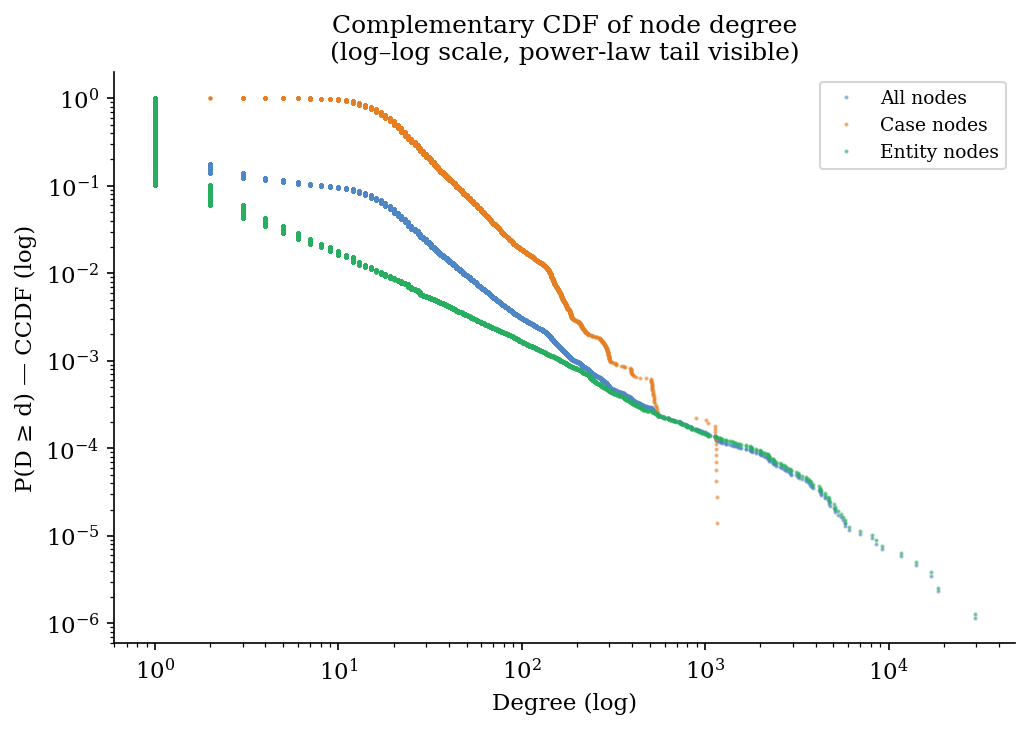
\includegraphics[width=\linewidth,height=0.55\textheight,keepaspectratio]{figures/37_degree_ccdf_loglog.png}

      \vspace{0.3em}
      \small
      The degree distribution is heavy-tailed: most nodes are leaves or near-leaves, while a small number of legal authorities act as super-hubs.
    \end{column}
  \end{columns}
\end{frame}

\begin{frame}{How the Legal Domains Connect}
  \scriptsize
  \begin{columns}[T]
    \begin{column}{0.58\textwidth}
      \centering
      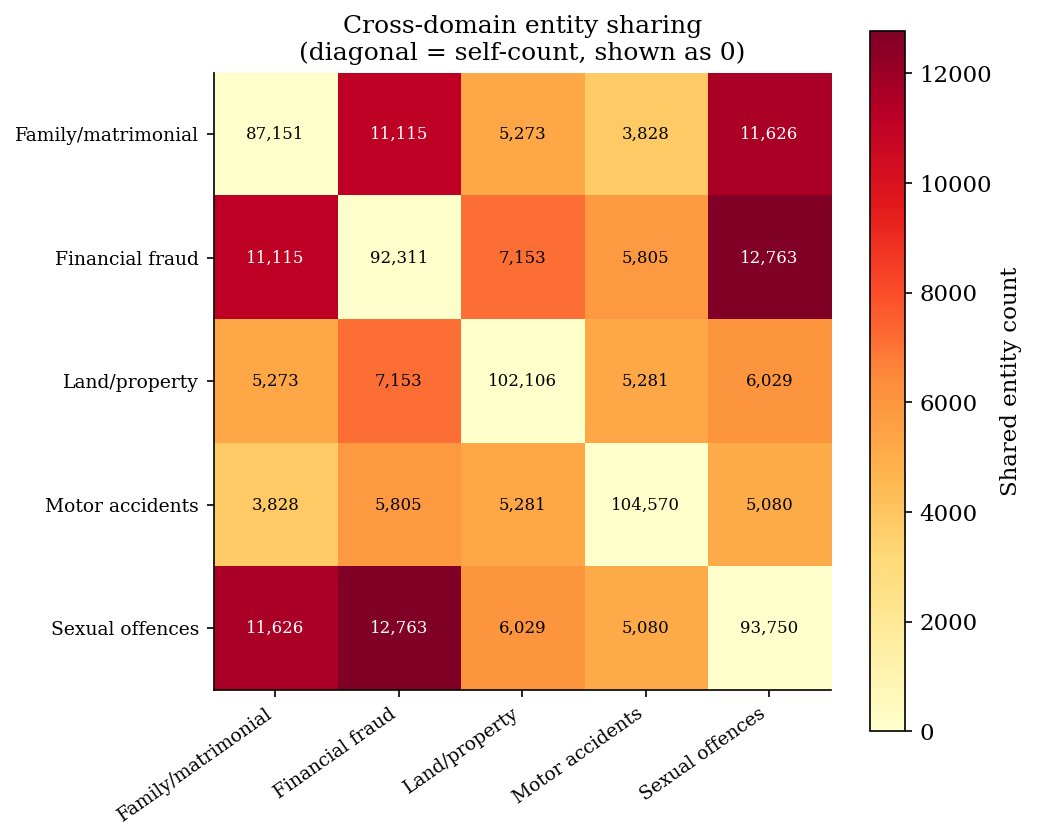
\includegraphics[width=\linewidth,height=0.52\textheight,keepaspectratio]{figures/20_cross_bucket_sharing_matrix.png}
    \end{column}
    \begin{column}{0.38\textwidth}
      \begin{block}{Main Pattern}
        \begin{tightitemize}
          \item Family, financial fraud, and sexual offences share heavily because they are IPC/CrPC-driven.
          \item Motor accidents shares moderately through procedural authorities and appellate courts.
          \item Land \& property is more weakly connected because it has a different statutory backbone.
        \end{tightitemize}
      \end{block}
      \small
      The domains are related enough for pooled training to matter, but different enough that transfer remains non-trivial.
    \end{column}
  \end{columns}
\end{frame}

\section{Model and Experimental Design}

\begin{frame}{Why HGT Instead of a Simpler GNN?}
  \begin{columns}[T]
    \begin{column}{0.56\textwidth}
      \begin{tightitemize}
        \item The graph has \highlight{many node types} with different feature semantics.
        \item It also has \highlight{many relation types}: \texttt{cites\_statute}, \texttt{heard\_in}, \texttt{belongs\_to\_statute}, \texttt{has\_petitioner}, and more.
        \item HGT gives:
        \begin{tightitemize}
          \item per-node-type projections,
          \item per-relation message functions,
          \item attention over typed neighbourhoods.
        \end{tightitemize}
        \item That makes it better suited than homogeneous GNNs or simple relation-shared models.
      \end{tightitemize}
    \end{column}
    \begin{column}{0.40\textwidth}
      \begin{block}{Architectural Intuition}
        A legal graph should not force statutes, arguments, parties, and courts into one shared geometry before message passing begins.
      \end{block}
      \begin{block}{Two-Layer Choice}
        Two HGT layers are enough to move information between a case and the shared legal authorities cited in its argument structure.
      \end{block}
    \end{column}
  \end{columns}
\end{frame}

\begin{frame}{Model Architecture}
  \centering
  \resizebox{0.96\textwidth}{!}{%
  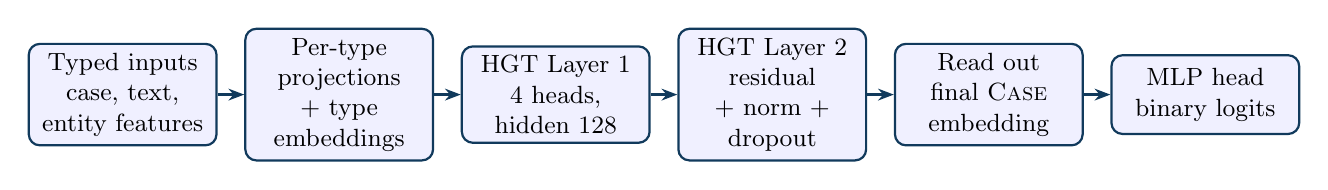
\begin{tikzpicture}[
    every node/.style={font=\small},
    box/.style={rectangle, rounded corners, draw=ThesisBlue, thick, fill=blue!6, minimum width=2.35cm, minimum height=1cm, align=center, text width=2.15cm},
    arrow/.style={-{Stealth[length=2mm]}, thick, draw=ThesisBlue}
  ]
    \node[box] (n1) at (0,0) {Typed inputs\\case, text, entity features};
    \node[box] (n2) at (2.75,0) {Per-type projections\\+ type embeddings};
    \node[box] (n3) at (5.50,0) {HGT Layer 1\\4 heads, hidden 128};
    \node[box] (n4) at (8.25,0) {HGT Layer 2\\residual + norm + dropout};
    \node[box] (n5) at (11.0,0) {Read out\\final \textsc{Case} embedding};
    \node[box] (n6) at (13.75,0) {MLP head\\binary logits};
    \draw[arrow] (n1) -- (n2);
    \draw[arrow] (n2) -- (n3);
    \draw[arrow] (n3) -- (n4);
    \draw[arrow] (n4) -- (n5);
    \draw[arrow] (n5) -- (n6);
  \end{tikzpicture}}

  \vspace{0.9em}
  \begin{columns}[T]
    \begin{column}{0.49\textwidth}
      \begin{block}{Training}
        AdamW, learning rate $10^{-3}$, weight decay $10^{-5}$, 60 epochs, early stopping by validation macro-F1, class-balanced cross-entropy.
      \end{block}
    \end{column}
    \begin{column}{0.47\textwidth}
      \begin{block}{Node Features}
        \texttt{bge-m3} text embeddings for text nodes, canonical-name embeddings plus scalar features for entity nodes, bucket metadata for case nodes.
      \end{block}
    \end{column}
  \end{columns}
\end{frame}

\begin{frame}{Experimental Protocol}
  \scriptsize
  \begin{block}{Evaluation Regime}
    \setlength{\tabcolsep}{4pt}
    \renewcommand{\arraystretch}{1.15}
    \begin{adjustbox}{max width=\textwidth}
      \begin{tabular}{p{3.3cm}p{10.7cm}}
        \toprule
        \textbf{Transductive setting} & the full graph (all nodes and edges) is built before any split. The model sees the entire graph topology --- including shared statutes, provisions, and precedents that span train and test cases --- but test labels are masked during training. This lets the GNN exploit the shared legal-authority structure without leaking outcomes. \\
        \midrule
        \textbf{5-fold cross-validation} & (seeds 42--46): the 71{,}813 cases are partitioned into 5 folds so that every case appears in a test set exactly once. This gives a variance estimate from 5 independent runs and ensures reported metrics cover the full dataset, not a single held-out slice. \\
        \midrule
        \textbf{Per-fold split} & 72\% train / 8\% val / 20\% test. \\
        \bottomrule
      \end{tabular}
    \end{adjustbox}
  \end{block}

  \vspace{0.4em}
  \begin{columns}[T,onlytextwidth]
    \begin{column}{0.49\textwidth}
      \begin{block}{Settings}
        \begin{tightitemize}
          \item 1 pooled cross-bucket setting (all 5 domains combined)
          \item 5 per-domain settings (one model per bucket)
          \item 1 zero-shot unseen-domain setting (food safety)
        \end{tightitemize}
      \end{block}
    \end{column}
    \begin{column}{0.49\textwidth}
      \begin{block}{Metrics}
        \begin{tightitemize}
          \item Primary: macro-F1
          \item Secondary: accuracy, ROC-AUC
          \item Supplementary: per-class precision/recall/F1
        \end{tightitemize}
      \end{block}
    \end{column}
  \end{columns}
\end{frame}

\begin{frame}{Per-Bucket Train / Val / Test Splits}
  \scriptsize
  \centering
  \begin{adjustbox}{max width=0.95\textwidth}
    \begin{tabular}{lrrrrrr}
      \toprule
       & & \multicolumn{3}{c}{\textbf{Per-fold sizes}} & \multicolumn{2}{c}{\textbf{Test class support}} \\
      \cmidrule(lr){3-5}\cmidrule(lr){6-7}
      \textbf{Bucket} & \textbf{Total} & \textbf{Train} & \textbf{Val} & \textbf{Test} & $|{-1}|$ & $|{+1}|$ \\
      \midrule
      Family \& Matrimonial & 14{,}771 & 10{,}636 & 1{,}181 & 2{,}954 & 988    & 1{,}966 \\
      Financial Fraud       & 14{,}158 & 10{,}194 & 1{,}132 & 2{,}832 & 1{,}120 & 1{,}711 \\
      Land \& Property      & 13{,}284 &  9{,}565 & 1{,}062 & 2{,}657 & 1{,}630 & 1{,}027 \\
      Motor Accidents       & 15{,}064 & 10{,}847 & 1{,}205 & 3{,}013 & 885    & 2{,}128 \\
      Sexual Offences       & 14{,}534 & 10{,}466 & 1{,}162 & 2{,}907 & 1{,}002 & 1{,}905 \\
      \midrule
      Cross-bucket pooled   & 71{,}813 & 51{,}705 & 5{,}745 & 14{,}363 & 5{,}625 & 8{,}737 \\
      \bottomrule
    \end{tabular}
  \end{adjustbox}

  \vspace{0.4em}
  \scriptsize 5-fold CV with seeds 42--46. Per-fold sizes are fold-0 representatives; folds vary by $\pm 1$ at the boundary. Class supports are averaged across folds. The pooled \emph{Total} is smaller than the 73{,}804 merged cases because procedural and unmapped labels are excluded from the binary task.
\end{frame}

\begin{frame}{Baselines}
  \scriptsize
  \centering
  \textbf{What each baseline is}\\[0.25em]
  \begin{adjustbox}{max width=0.98\textwidth}
    \begin{tabular}{p{2.4cm}p{11.0cm}}
      \toprule
      \textbf{Baseline} & \textbf{Description} \\
      \midrule
      Majority & Always predicts the dominant class --- trivial lower bound, no learning. \\
      LR (no graph) & Logistic regression on BGE-M3 text embedding $+$ 12 scalar features. No graph, no message passing --- measures what text alone achieves. \\
      \texttt{baseline} HGT & Full 17-node-type reasoning graph, statutes/provisions/precedents shared across cases. Reference point for all graph variants. \\
      \bottomrule
    \end{tabular}
  \end{adjustbox}

  \vspace{0.8em}
  \textbf{Results (5-fold, cross-bucket)}\\[0.25em]
  \begin{adjustbox}{max width=0.78\textwidth}
    \begin{tabular}{lcc}
      \toprule
      \textbf{Baseline} & \textbf{Accuracy} & \textbf{Macro-F1} \\
      \midrule
      Majority           & 0.6083 $\pm$ 0.0000 & 0.3782 $\pm$ 0.0000 \\
      LR (no graph)      & 0.7432 $\pm$ 0.0032 & 0.7359 $\pm$ 0.0034 \\
      \texttt{baseline} HGT & 0.7811 $\pm$ 0.0055 & 0.7759 $\pm$ 0.0043 \\
      \bottomrule
    \end{tabular}
  \end{adjustbox}

  \vspace{0.5em}
  \scriptsize All rows are 5-fold means $\pm$ std. Every one of the 71{,}813 cases appears in a test fold exactly once --- LR and HGT results are directly comparable.\\[0.25em]
  \highlight{LR $\rightarrow$ HGT: $+4.0$ pts macro-F1} --- the honest ``what does the graph buy us'' delta.
\end{frame}

\begin{frame}{What Each Experimental Variant Tests}
  \tiny
  \setlength{\tabcolsep}{4pt}
  \begin{tabular}{p{2.6cm}p{2.0cm}p{8.5cm}}
    \toprule
    \textbf{Variant} & \textbf{Type} & \textbf{What It Changes / What It Measures} \\
    \midrule
    \texttt{text\_only} & graph ablation & Same two-layer HGT, but the graph is reduced to the case node plus the text-section nodes (preamble, facts, arguments, petitioner/respondent/other-lawyer args). \textbf{Removes the entity layer only} --- still graph-based, still message-passing. Isolates the contribution of the entity/authority layer. \\
    \texttt{hierarchical\_enc} & encoder change & Same graph as baseline, but long sections re-encoded with \textbf{hierarchical \texttt{bge-m3} chunking} (1800-char chunks, 200-char overlap). Tests whether richer long-document text representation helps. \\
    \texttt{section\_sep\_enc} & encoder change & Each rhetorical section (preamble, facts, arguments, party-side arguments) keeps its \textbf{own typed text node and its own embedding} instead of being collapsed into the case representation. \\
    \texttt{party\_args\_lr\_decay} & training + features & Adds \textbf{petitioner and respondent argument streams} to the case-side text features, plus a \texttt{reduce\_on\_plateau} LR schedule (90 epochs, patience 20, decay 0.5). Tests whether stabilising the argument stream and the optimisation schedule helps. \\
    \texttt{no\_names} & leakage ablation & \textbf{Removes party / judge / lawyer / court node types} and their scalar counts from the graph. Directly measures whether identity nodes were acting as a shortcut. \\
    \texttt{no\_cross\_case} & structural ablation & \textbf{Disables cross-case sharing}: every statute, provision, and precedent becomes a per-case copy. Measures the contribution of shared legal-authority bridges. \\
    \texttt{case\_node\_minimised} & structural ablation & Case node carries \textbf{only its 12 scalar features}; no text embedding is concatenated into it. Forces the GNN to reconstruct the case representation from the section and entity nodes alone. \\
    \bottomrule
  \end{tabular}
\end{frame}

\section{Prediction Results}

\begin{frame}{Headline: Macro-F1 Across All Variants and Domains}
  \tiny
  \centering
  \setlength{\tabcolsep}{3pt}
  \begin{adjustbox}{max width=\textwidth}
    \begin{tabular}{lccccccc}
      \toprule
      \textbf{Model} & \textbf{Family} & \textbf{Fin.\ Fraud} & \textbf{Land/Prop.} & \textbf{Motor Acc.} & \textbf{Sexual Off.} & \textbf{Cross-bucket} & \textbf{Mean$_5$} \\
      \midrule
      \texttt{LR (no graph)}$^\dagger$          & 0.7583               & 0.6961               & 0.7184               & 0.7622               & 0.6977               & 0.7372               & 0.7265 \\
      \texttt{text\_only} (graph $-$ entities)  & 0.8025\,$\pm$\,0.008 & 0.7535\,$\pm$\,0.006 & 0.7883\,$\pm$\,0.011 & 0.7954\,$\pm$\,0.005 & 0.7544\,$\pm$\,0.007 & 0.7671\,$\pm$\,0.005 & 0.7788 \\
      \texttt{baseline} (HGT)                   & 0.8042\,$\pm$\,0.009 & 0.7577\,$\pm$\,0.010 & 0.7916\,$\pm$\,0.006 & 0.8147\,$\pm$\,0.005 & 0.7538\,$\pm$\,0.007 & 0.7759\,$\pm$\,0.004 & 0.7844 \\
      \texttt{hierarchical\_enc}                & \runnerup{\underline{0.8073\,$\pm$\,0.009}} & 0.7570\,$\pm$\,0.011 & 0.7908\,$\pm$\,0.010 & 0.8157\,$\pm$\,0.011 & \runnerup{\underline{0.7557\,$\pm$\,0.005}} & 0.7754\,$\pm$\,0.003 & 0.7853 \\
      \texttt{section\_sep\_enc}                & \best{0.8077\,$\pm$\,0.010} & \best{0.7631\,$\pm$\,0.014} & 0.7947\,$\pm$\,0.009 & 0.8158\,$\pm$\,0.003 & 0.7540\,$\pm$\,0.007 & \runnerup{\underline{0.7831\,$\pm$\,0.009}} & \best{0.7871} \\
      \best{\texttt{party\_args\_lr\_decay}}    & 0.8056\,$\pm$\,0.004 & 0.7579\,$\pm$\,0.011 & \runnerup{\underline{0.7951\,$\pm$\,0.005}} & 0.8164\,$\pm$\,0.006 & \best{0.7596\,$\pm$\,0.004} & \best{0.7959\,$\pm$\,0.003} & 0.7869 \\
      \texttt{no\_names}                        & 0.8066\,$\pm$\,0.006 & \runnerup{\underline{0.7599\,$\pm$\,0.011}} & \best{0.7957\,$\pm$\,0.012} & \best{0.8192\,$\pm$\,0.005} & 0.7537\,$\pm$\,0.008 & 0.7797\,$\pm$\,0.007 & \runnerup{\underline{0.7870}} \\
      \texttt{no\_cross\_case}                  & 0.8058\,$\pm$\,0.009 & 0.7580\,$\pm$\,0.013 & 0.7941\,$\pm$\,0.008 & 0.8146\,$\pm$\,0.006 & 0.7521\,$\pm$\,0.008 & 0.7767\,$\pm$\,0.003 & 0.7849 \\
      \texttt{case\_node\_minimised}            & 0.8006\,$\pm$\,0.005 & 0.7575\,$\pm$\,0.010 & 0.7862\,$\pm$\,0.006 & \runnerup{\underline{0.8192\,$\pm$\,0.010}} & 0.7514\,$\pm$\,0.006 & 0.7697\,$\pm$\,0.002 & 0.7830 \\
      \bottomrule
    \end{tabular}
  \end{adjustbox}

  \vspace{0.5em}
  \scriptsize Mean $\pm$ std over 5 folds for HGT variants. \best{Bold} = best per column; \runnerup{\underline{underline}} = second best. \textbf{Mean$_5$} = unweighted average across the five per-domain columns (excludes cross-bucket).\\
  $^\dagger$\,\texttt{LR (no graph)}: logistic regression on BGE-M3 case-text embedding $+$ 12 scalar case features --- no graph, no message passing. Reported on fold 0 from the probing pipeline. The gap between this row and the HGT rows is the actual ``what does the graph buy us'' delta: $\sim$\,$+6$ pts macro-F1 on the pooled task and $+5$--$10$ pts per bucket.
\end{frame}

\begin{frame}{Ablation $\Delta$: Macro-F1 Change vs.\ HGT Baseline}
  \scriptsize
  \centering
  \setlength{\tabcolsep}{4pt}
  \begin{adjustbox}{max width=\textwidth}
    \begin{tabular}{lcccccc}
      \toprule
      \textbf{Variant} & \textbf{Family} & \textbf{Fin.\ Fraud} & \textbf{Land/Prop.} & \textbf{Motor Acc.} & \textbf{Sexual Off.} & \textbf{Cross-bucket} \\
      \midrule
      \texttt{text\_only}                       & $-0.0017\,\downarrow$ & $-0.0042\,\downarrow$ & $-0.0033\,\downarrow$ & $-0.0193\,\downarrow$ & $+0.0006\,\uparrow$  & $-0.0088\,\downarrow$ \\
      \texttt{hierarchical\_enc}                & $+0.0031\,\uparrow$   & $-0.0007\,\downarrow$ & $-0.0008\,\downarrow$ & $+0.0010\,\uparrow$   & $+0.0019\,\uparrow$  & $-0.0005\,\downarrow$ \\
      \texttt{section\_sep\_enc}                & $+0.0035\,\uparrow$   & $+0.0054\,\uparrow$   & $+0.0031\,\uparrow$   & $+0.0011\,\uparrow$   & $+0.0002\,\uparrow$  & $+0.0072\,\uparrow$   \\
      \best{\texttt{party\_args\_lr\_decay}}    & $+0.0014\,\uparrow$   & $+0.0002\,\uparrow$   & $+0.0035\,\uparrow$   & $+0.0017\,\uparrow$   & $+0.0058\,\uparrow$  & \best{$+0.0200\,\uparrow$} \\
      \texttt{no\_names}                        & $+0.0024\,\uparrow$   & $+0.0022\,\uparrow$   & $+0.0041\,\uparrow$   & $+0.0045\,\uparrow$   & $-0.0001\,\downarrow$ & $+0.0038\,\uparrow$   \\
      \texttt{no\_cross\_case}                  & $+0.0016\,\uparrow$   & $+0.0003\,\uparrow$   & $+0.0025\,\uparrow$   & $-0.0001\,\downarrow$ & $-0.0017\,\downarrow$ & $+0.0008\,\uparrow$   \\
      \texttt{case\_node\_minimised}            & $-0.0036\,\downarrow$ & $-0.0002\,\downarrow$ & $-0.0054\,\downarrow$ & $+0.0045\,\uparrow$   & $-0.0024\,\downarrow$ & $-0.0062\,\downarrow$ \\
      \bottomrule
    \end{tabular}
  \end{adjustbox}

  \vspace{0.6em}
  \begin{tightitemize}
    \item Removing the entity layer (\texttt{text\_only}, still HGT over case + text sections) is the single largest drop, especially on motor accidents ($-1.9$ pts) and on the pooled task ($-0.9$ pts) --- so the entity layer measurably contributes on top of the text-only graph.
    \item Adding the petitioner/respondent argument streams plus an LR-decay schedule yields the largest pooled gain ($+2.0$ pts macro-F1).
    \item \texttt{no\_names} is at or above baseline on every bucket --- direct evidence against identity-as-shortcut.
    \item Many per-bucket deltas are within $\pm 0.005$, so on individual domains several variants should be read as a cluster rather than a strict ranking.
    \item For the actual ``does the graph help over no graph'' delta, see the headline table's \texttt{LR (no graph)} row: the gap to the best HGT variant is $\sim$\,$+6$ pts macro-F1 on the pooled task.
  \end{tightitemize}
\end{frame}

\begin{frame}{Per-Class Behaviour on the Pooled Cross-Bucket Test Set}
  \scriptsize
  \centering
  \setlength{\tabcolsep}{5pt}
  \begin{adjustbox}{max width=\textwidth}
    \begin{tabular}{lcccccc}
      \toprule
       & \multicolumn{3}{c}{\textbf{Class $-1$ (appellant lost)}} & \multicolumn{3}{c}{\textbf{Class $+1$ (appellant won)}} \\
      \cmidrule(lr){2-4}\cmidrule(lr){5-7}
      \textbf{Model} & \textbf{P} & \textbf{R} & \textbf{F1} & \textbf{P} & \textbf{R} & \textbf{F1} \\
      \midrule
      \texttt{text\_only}                       & 0.685 & 0.782          & 0.730 & 0.846          & 0.768 & 0.805 \\
      \texttt{baseline} (HGT)                   & 0.690 & \textbf{0.805} & 0.742 & 0.860          & 0.765 & 0.810 \\
      \texttt{hierarchical\_enc}                & 0.692 & 0.795          & 0.740 & 0.854          & 0.772 & 0.811 \\
      \texttt{section\_sep\_enc}                & 0.705 & 0.796          & 0.747 & 0.857          & 0.785 & 0.819 \\
      \textbf{\texttt{party\_args\_lr\_decay}}  & \textbf{0.723} & \underline{0.803} & \textbf{0.761} & \textbf{0.864} & \textbf{0.801} & \textbf{0.831} \\
      \texttt{no\_names}                        & 0.707 & 0.779          & 0.741 & 0.848          & 0.792 & 0.819 \\
      \texttt{no\_cross\_case}                  & 0.704 & 0.777          & 0.738 & 0.846          & 0.788 & 0.816 \\
      \texttt{case\_node\_minimised}            & 0.686 & 0.788          & 0.733 & 0.849          & 0.767 & 0.806 \\
      \bottomrule
    \end{tabular}
  \end{adjustbox}

  \vspace{0.5em}
  \scriptsize Class supports per fold: $|{-1}|\!\approx\!5{,}625$, $|{+1}|\!\approx\!8{,}737$. The minority class $-1$ is consistently the harder one (lower precision across all variants); \texttt{party\_args\_lr\_decay} is the only variant that lifts both classes simultaneously, including a $+3.3$-pt jump in $-1$ precision over baseline.
\end{frame}

\begin{frame}{What the Ablations Actually Say}
  \tiny
  \begin{block}{Six Concrete Findings}
    \begin{tightitemize}
      \item \highlight{Graph beats no-graph by $\sim$\,$+6$ pts macro-F1} on the pooled task (LR 0.737 $\rightarrow$ best variant 0.796). Decomposed: case--section graph alone ($+0.030$) $\gg$ entity layer ($+0.009$) $<$ encoder/optimisation refinements ($+0.020$). The biggest single jump is the graph itself, not the deeper variants.
      \item \highlight{Identity is removable}: \texttt{no\_names} is at or above baseline on every bucket --- direct evidence against name leakage. Notably, \texttt{no\_names} is the \emph{best} HGT variant on Land/Property and Motor Accidents, suggesting party/judge nodes can even add noise on some domains.
      \item \highlight{Cross-case sharing helps modestly in transductive training}: \texttt{no\_cross\_case} is within $\pm 0.005$ of baseline on most buckets; in-bucket sharing already gives the model enough connectivity.
      \item \highlight{Encoder organisation matters per domain}: \texttt{section\_sep\_enc} / \texttt{hierarchical\_enc} dominate ROC-AUC on Family, Fin.\ Fraud, Land/Prop, Motor Acc.\ --- but lose to \texttt{party\_args\_lr\_decay} on macro-F1 once class balance is taken into account.
      \item \highlight{Best pooled model wins the hardest tasks}: \texttt{party\_args\_lr\_decay} dominates the pooled setting and the two hardest domains (Sexual Off., Fin.\ Fraud), with $+2.0$ pts macro-F1 over baseline.
      \item \highlight{The pooled optimum is not the universal optimum}: no single variant wins every per-bucket column; on individual domains several variants form a cluster within $\pm 0.005$.
    \end{tightitemize}
  \end{block}
  \begin{block}{Per-Class Finding}
    The \highlight{minority class is the binding constraint} in every bucket (lowest F1 in the per-class table; minority is $-1$ in four buckets and $+1$ in Land/Property). \texttt{party\_args\_lr\_decay} is the only variant that lifts \emph{both} classes simultaneously --- $+3.3$ pts P($-1$) and $+3.6$ pts R($+1$) over baseline --- which is what produces its pooled gain.
  \end{block}
\end{frame}

\begin{frame}{Best Model (\texttt{party\_args\_lr\_decay}): Per-Bucket Per-Class Breakdown}
  \scriptsize
  \centering
  \setlength{\tabcolsep}{5pt}
  \begin{adjustbox}{max width=\textwidth}
    \begin{tabular}{lcccccccc}
      \toprule
       & \multicolumn{4}{c}{\textbf{Class $-1$ (lost)}} & \multicolumn{4}{c}{\textbf{Class $+1$ (won)}} \\
      \cmidrule(lr){2-5}\cmidrule(lr){6-9}
      \textbf{Bucket} & \textbf{P} & \textbf{R} & \textbf{F1} & \textbf{Sup.} & \textbf{P} & \textbf{R} & \textbf{F1} & \textbf{Sup.} \\
      \midrule
      Family \& Matrimonial & 0.731 & 0.758 & 0.744 & 988    & 0.876 & 0.859 & 0.868 & 1{,}966 \\
      Financial Fraud       & 0.724 & 0.682 & 0.702 & 1{,}120 & 0.799 & 0.829 & 0.814 & 1{,}711 \\
      Land \& Property      & 0.823 & 0.881 & 0.851 & 1{,}630 & 0.790 & 0.698 & 0.740 & 1{,}027 \\
      Motor Accidents       & 0.700 & 0.806 & 0.749 & 885    & 0.914 & 0.856 & 0.884 & 2{,}128 \\
      Sexual Offences       & 0.676 & 0.704 & 0.689 & 1{,}002 & 0.841 & 0.821 & 0.831 & 1{,}905 \\
      \midrule
      Cross-bucket pooled   & 0.723 & 0.803 & 0.761 & 5{,}625 & 0.864 & 0.801 & 0.831 & 8{,}737 \\
      \bottomrule
    \end{tabular}
  \end{adjustbox}

  \vspace{0.6em}
  \begin{columns}[T]
    \begin{column}{0.50\textwidth}
      \begin{block}{Difficulty Ordering (Macro-F1)}
        \begin{tightitemize}
          \item easiest: \highlight{Motor Accidents} (0.816)
          \item then: Family / Land \& Property
          \item hardest: \highlight{Sexual Offences} (0.760), \highlight{Financial Fraud} (0.758)
        \end{tightitemize}
      \end{block}
    \end{column}
    \begin{column}{0.46\textwidth}
      \begin{block}{Where the Model Wins / Loses}
        \begin{tightitemize}
          \item \highlight{Land \& Property} flips the imbalance: $-1$ is the majority class, and the model's $-1$ F1 (0.851) is the highest of any cell in the table.
          \item \highlight{Sexual Offences} has the lowest minority-class F1 (0.689) --- consistent with noisier outcome labels in that bucket.
          \item Motor Accidents has the highest $+1$ F1 (0.884), reflecting its repetitive statutory backbone.
        \end{tightitemize}
      \end{block}
    \end{column}
  \end{columns}
\end{frame}

% \begin{frame}{Zero-Shot Transfer to a Fully Unseen Legal Domain}
%   \scriptsize
%   \begin{columns}[T]
%     \begin{column}{0.58\textwidth}
%       \scriptsize
%       \begin{adjustbox}{max width=\linewidth}
%         \begin{tabular}{lcccc}
%           \toprule
%           \textbf{Setting} & \textbf{$N$} & \textbf{Accuracy} & \textbf{Macro-F1} & \textbf{ROC-AUC} \\
%           \midrule
%           Majority baseline (food safety) & 11{,}769 & 0.543 & -- & -- \\
%           Cross-bucket $\rightarrow$ food safety & 11{,}769 & 0.6079 $\pm$ 0.0054 & 0.6034 $\pm$ 0.0070 & 0.6749 $\pm$ 0.0198 \\
%           \midrule
%           In-domain pooled reference & 72{,}735 & 0.8020 $\pm$ 0.0036 & 0.7959 $\pm$ 0.0028 & 0.8831 \\
%           \bottomrule
%         \end{tabular}
%       \end{adjustbox}
%     \end{column}
%     \begin{column}{0.38\textwidth}
%       \begin{block}{What This Means}
%         \begin{tightitemize}
%           \item No fine-tuning was used.
%           \item Accuracy is \highlight{6.5 points above} the majority baseline.
%           \item The model clearly loses substantial performance out of domain.
%           \item But the transfer is non-trivial and stable across folds.
%         \end{tightitemize}
%       \end{block}
%       \begin{block}{Interpretation}
%         The pooled model learns a \highlight{partially domain-general legal prior}, not just a memorized list of the training buckets' statutes.
%       \end{block}
%     \end{column}
%   \end{columns}
% \end{frame}

\begin{frame}{Zero-Shot Transfer to a Fully Unseen Legal Domain}
  \scriptsize
  The model trained on the 5 pooled buckets (family, fraud, land, motor, sexual offences) was applied \highlight{without any fine-tuning} to \highlight{11{,}769 food-safety cases} --- a domain it had never seen. The food-safety graph was built with the same pipeline and the trained weights were loaded directly; only the test labels were evaluated.

  \vspace{0.8em}
  \centering
  \begin{adjustbox}{max width=0.82\textwidth}
    \begin{tabular}{lcccc}
      \toprule
      \textbf{Setting} & \textbf{$N$} & \textbf{Accuracy} & \textbf{Macro-F1} & \textbf{ROC-AUC} \\
      \midrule
      Majority baseline (food safety)       & 11{,}769 & 0.543              & ---                    & --- \\
      Cross-bucket $\rightarrow$ food safety & 11{,}769 & 0.6079 $\pm$ 0.0054 & 0.6034 $\pm$ 0.0070 & 0.6749 $\pm$ 0.0198 \\
      % \midrule
      % In-domain pooled reference             & 72{,}735 & 0.8020 $\pm$ 0.0036 & 0.7959 $\pm$ 0.0028 & 0.8831 \\
      \bottomrule
    \end{tabular}
  \end{adjustbox}

  \vspace{0.8em}
  \raggedright
  \begin{tightitemize}
    \item The zero-shot model sits \highlight{$+6.5$ pts accuracy above the food-safety majority baseline} and holds stable across all 5 folds (std $\pm 0.005$), suggesting the pooled model has learned a \highlight{partially domain-general legal prior} --- not just a memorised mapping of the training buckets' statutes --- though substantial performance is lost relative to in-domain.
  \end{tightitemize}
\end{frame}


\section{Interpretability and Error Analysis}

\begin{frame}{Interpretability Stack}
  \scriptsize
  \begin{columns}[T]
    \begin{column}{0.52\textwidth}
      \begin{block}{Four Levels of Interpretation}
        \begin{tightitemize}
          \item \highlight{Representation level}: what changed after graph message passing?
          \item \highlight{Component level}: which node and edge types matter?
          \item \highlight{Error level}: where does the model fail?
          \item \highlight{Case level}: why did one prediction happen?
        \end{tightitemize}
      \end{block}
      \begin{block}{Case-Level Pipeline}
        Frozen inference $\rightarrow$ FAISS retrieval index $\rightarrow$ heterogeneous PGExplainer $\rightarrow$ ranked legal evidence $\rightarrow$ LLM verbalisation.
      \end{block}
    \end{column}
    \begin{column}{0.44\textwidth}
      \scriptsize
      \begin{adjustbox}{max width=\linewidth}
        \begin{tabular}{p{1.5cm}p{2.7cm}p{3.6cm}}
          \toprule
          \textbf{Phase} & \textbf{Script} & \textbf{Output} \\
          \midrule
          1--2 & inference + index & embeddings, predictions, FAISS index \\
          3 & explainer training & hetero PGExplainer \\
          4 & importance extraction & ranked statutes, provisions, precedents, arguments \\
          5 & LLM translation & grounded natural-language explanation \\
          \bottomrule
        \end{tabular}
      \end{adjustbox}
    \end{column}
  \end{columns}
\end{frame}

\begin{frame}{What Did the GNN Learn Beyond the Raw Features?}
  \begin{columns}[T]
    \begin{column}{0.42\textwidth}
      \scriptsize
      \begin{tabular}{lcc}
        \toprule
        \textbf{Probe Input} & \textbf{Acc.} & \textbf{Macro-F1} \\
        \midrule
        Majority baseline & 0.6083 & 0.3782 \\
        Pre-GNN raw features & 0.7443 & 0.7372 \\
        Post-GNN embedding & 0.7840 & 0.7792 \\
        \bottomrule
      \end{tabular}

      \vspace{0.9em}
      \begin{block}{Key Point}
        The post-GNN representation is \highlight{16$\times$ smaller} than the pre-GNN raw feature vector, yet it is almost \highlight{4 points more accurate}. The gain comes from message passing, not probe capacity.
      \end{block}
    \end{column}
    \begin{column}{0.54\textwidth}
      \centering
      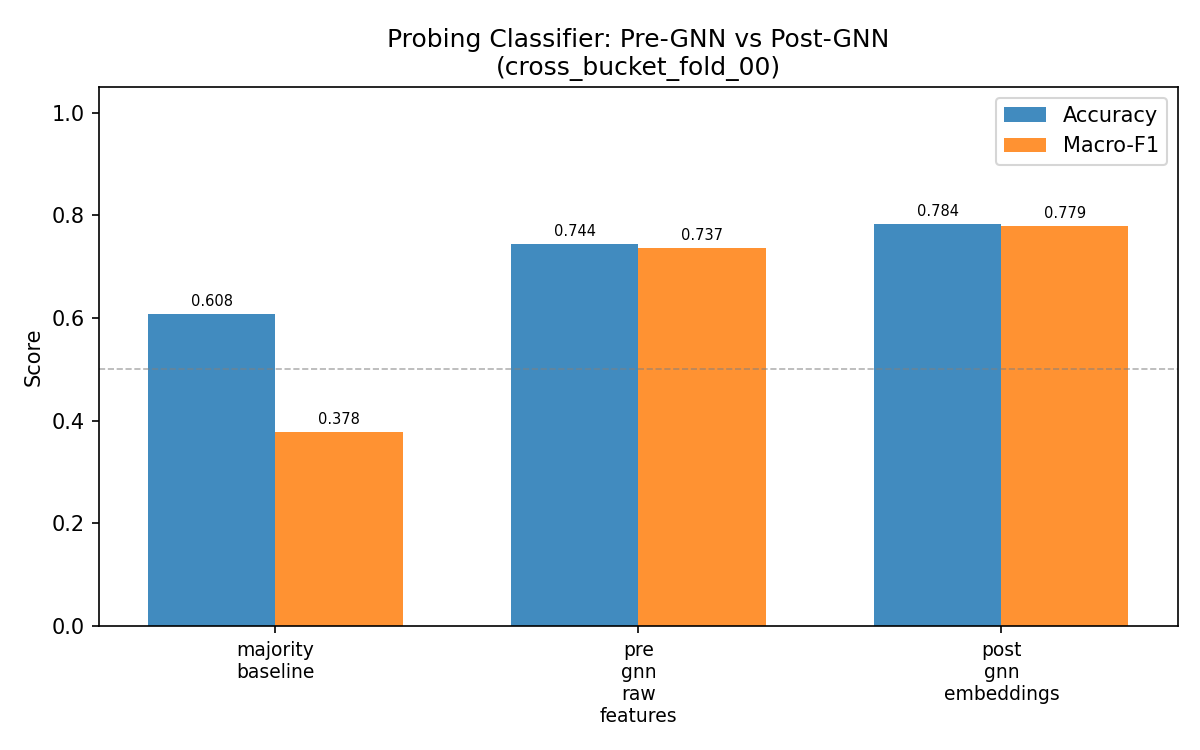
\includegraphics[width=\linewidth]{figures/explainability/probing_bar.png}
    \end{column}
  \end{columns}
\end{frame}

\begin{frame}{Embedding Geometry: Domain Structure}
  \centering
  \begin{columns}[T]
    \begin{column}{0.48\textwidth}
      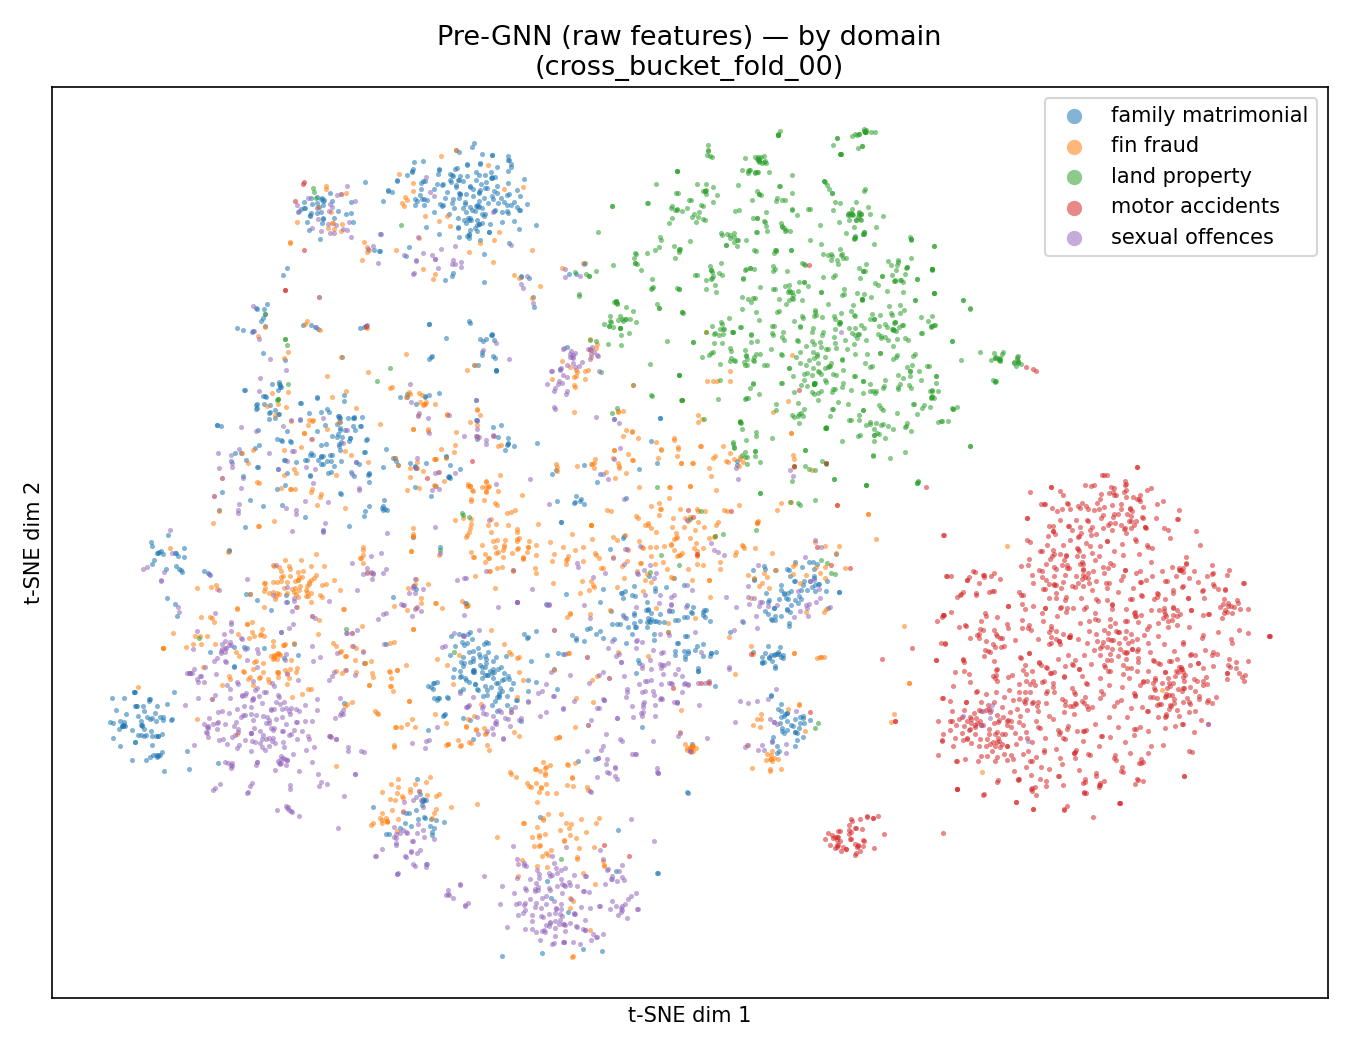
\includegraphics[width=\linewidth]{figures/explainability/tsne_pre_by_domain.png}
      \vspace{0.2em}
      \small Pre-GNN embeddings colored by domain
    \end{column}
    \begin{column}{0.48\textwidth}
      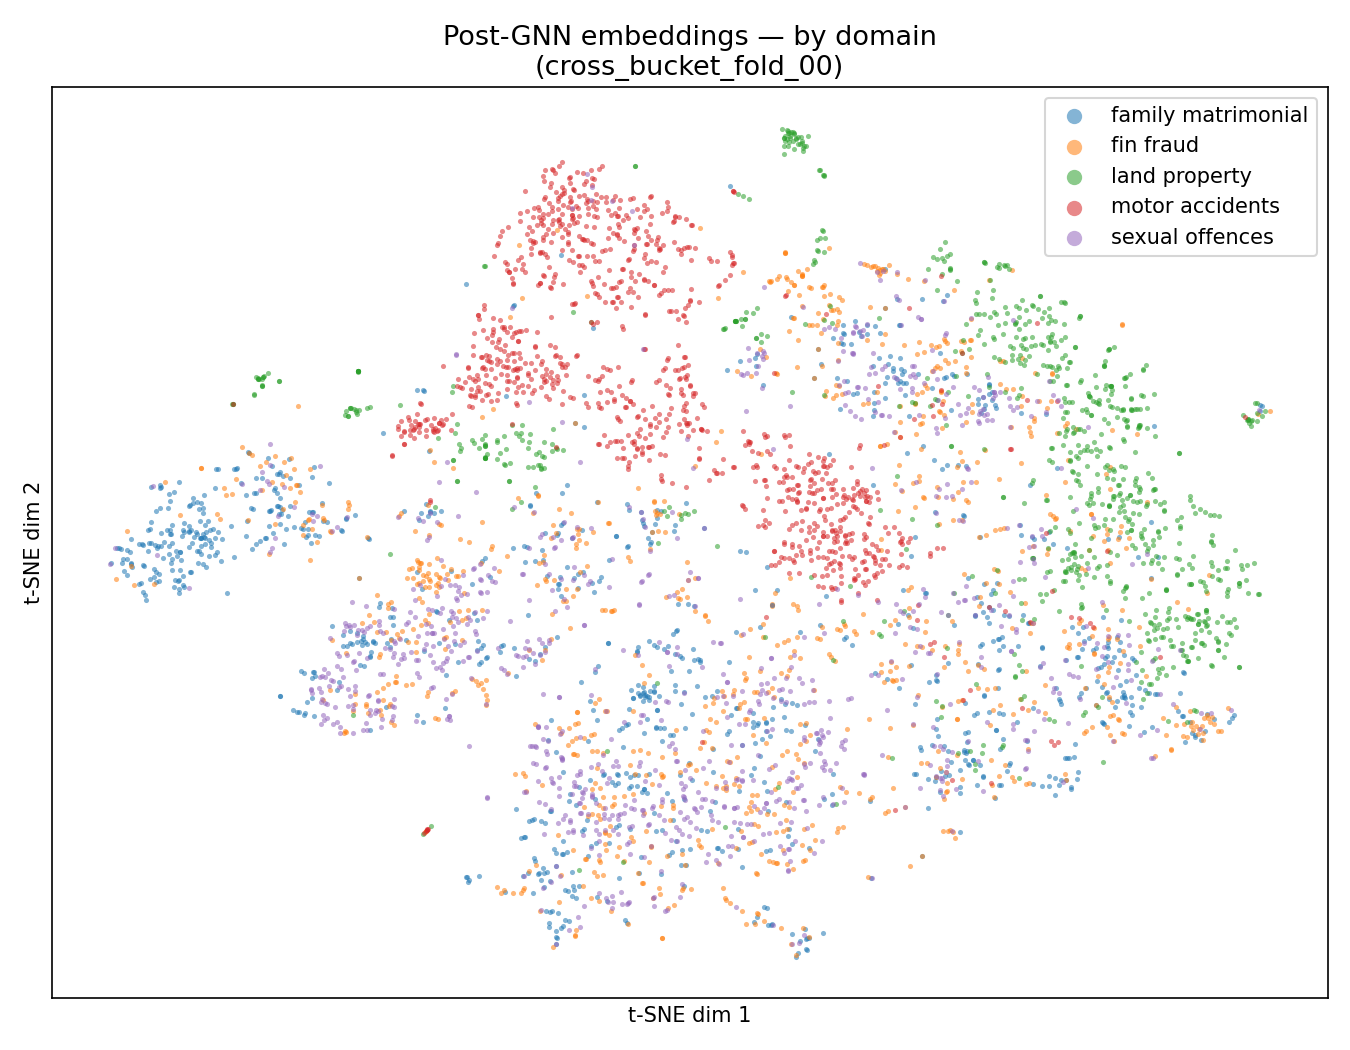
\includegraphics[width=\linewidth]{figures/explainability/tsne_post_by_domain.png}
      \vspace{0.2em}
      \small Post-GNN embeddings colored by domain
    \end{column}
  \end{columns}

  \vspace{0.6em}
  \small
  Domain structure is already present before message passing, which shows that raw legal text is informative about legal area.
\end{frame}

\begin{frame}{Embedding Geometry: Outcome Structure}
  \centering
  \begin{columns}[T]
    \begin{column}{0.48\textwidth}
      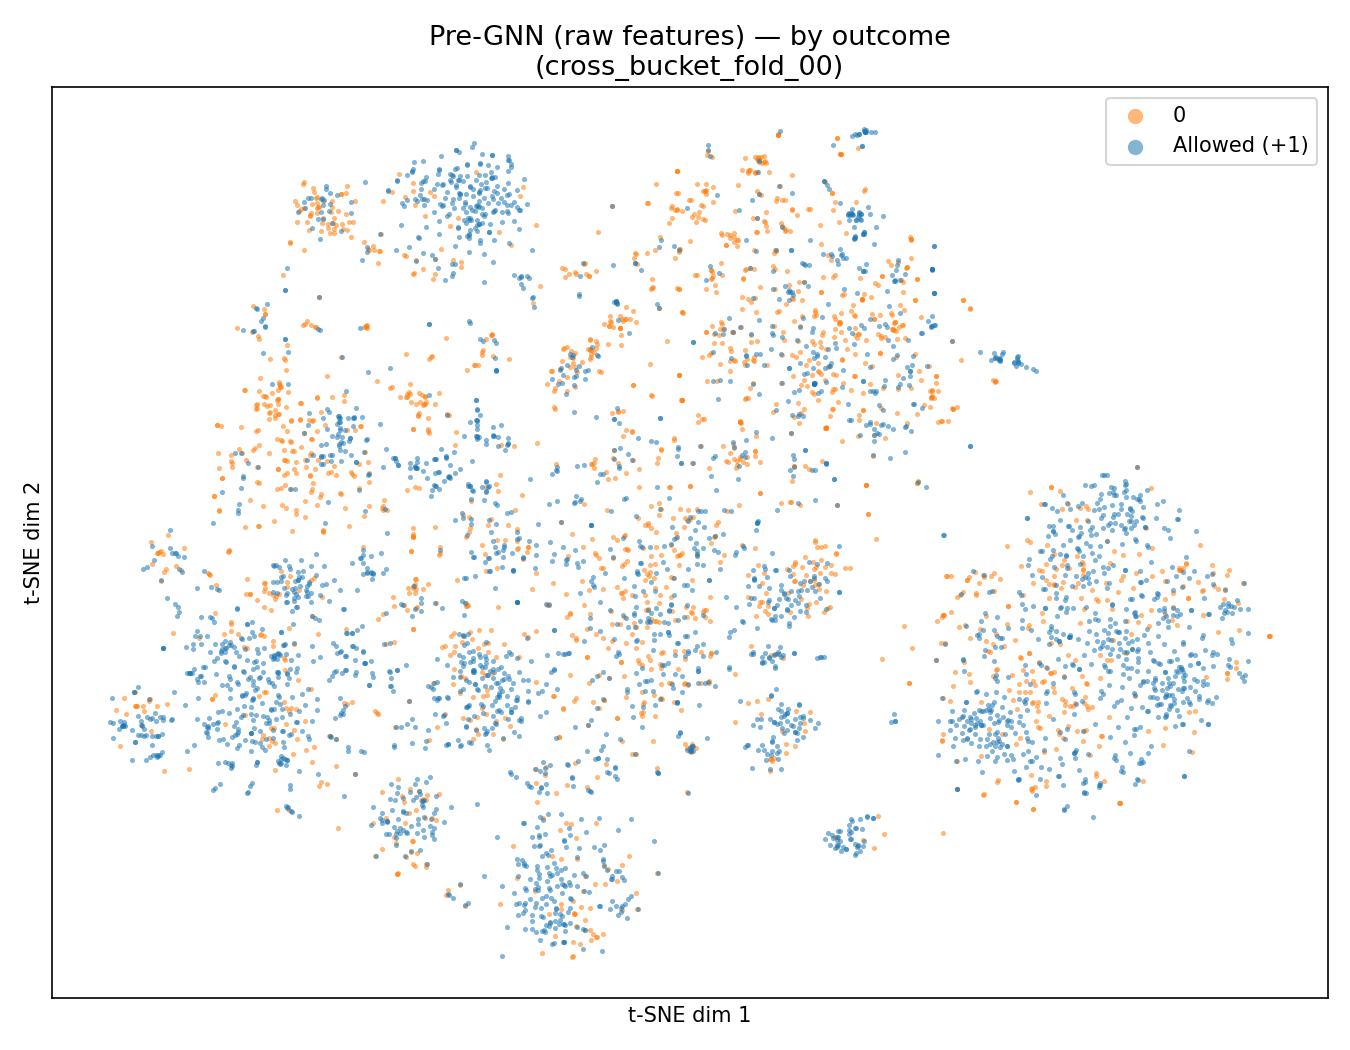
\includegraphics[width=\linewidth]{figures/explainability/tsne_pre_by_label.png}
      \vspace{0.2em}
      \small Pre-GNN embeddings colored by outcome
    \end{column}
    \begin{column}{0.48\textwidth}
      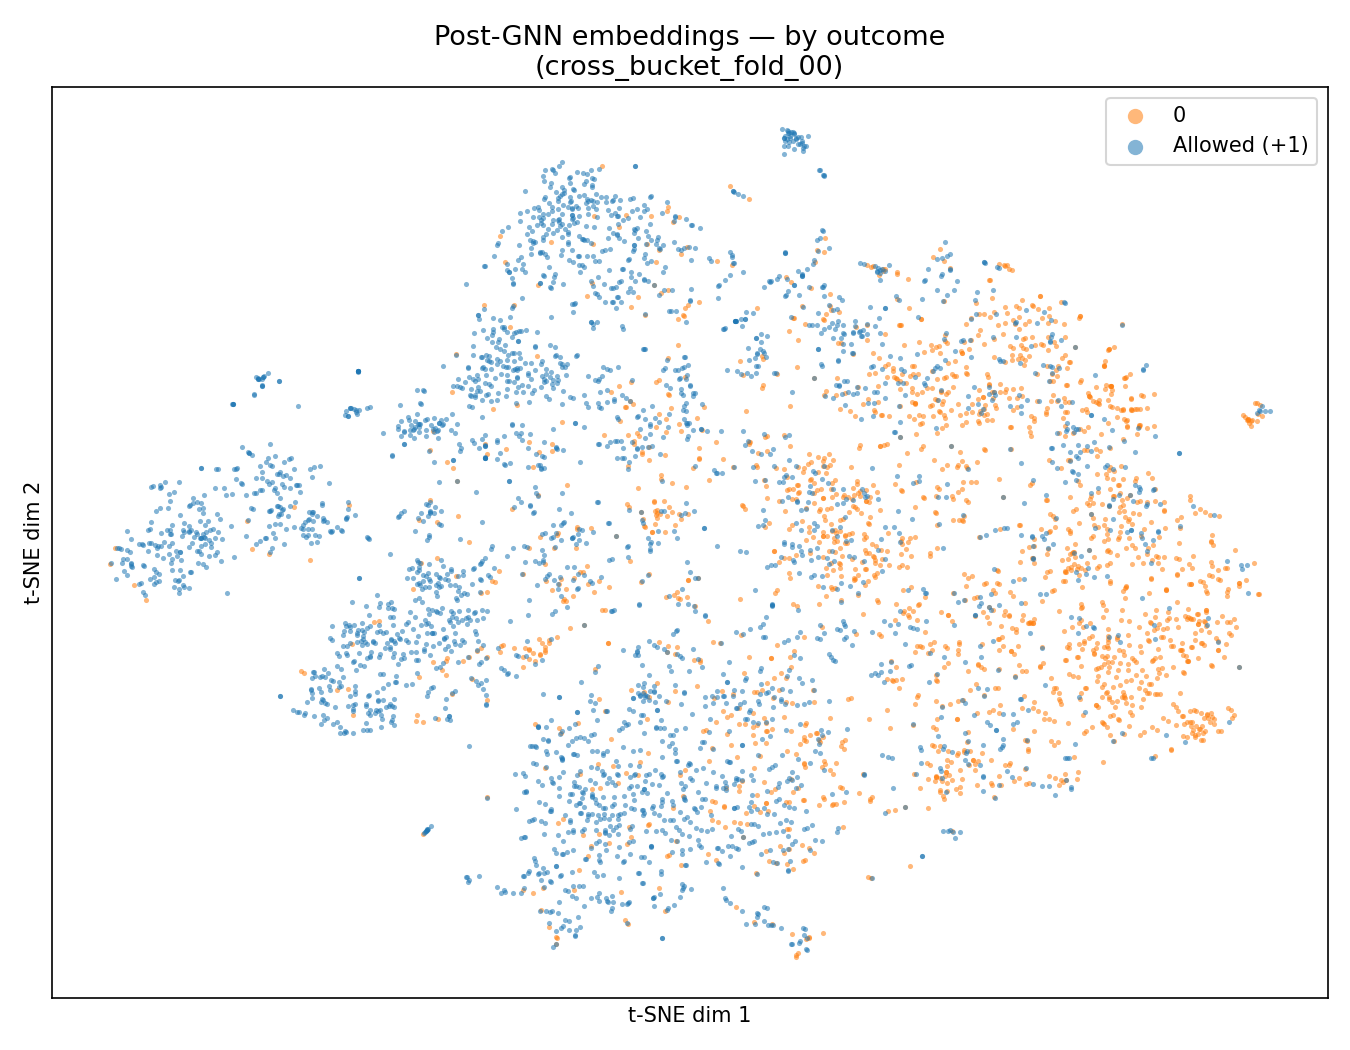
\includegraphics[width=\linewidth]{figures/explainability/tsne_post_by_label.png}
      \vspace{0.2em}
      \small Post-GNN embeddings colored by outcome
    \end{column}
  \end{columns}

  \vspace{0.6em}
  \small
  After message passing, outcome structure becomes much more visible \highlight{within} domain neighbourhoods. This is the geometric view of the graph's contribution.
\end{frame}

\begin{frame}{Node-Type Importance}
  \begin{columns}[T]
    \begin{column}{0.48\textwidth}
      \centering
      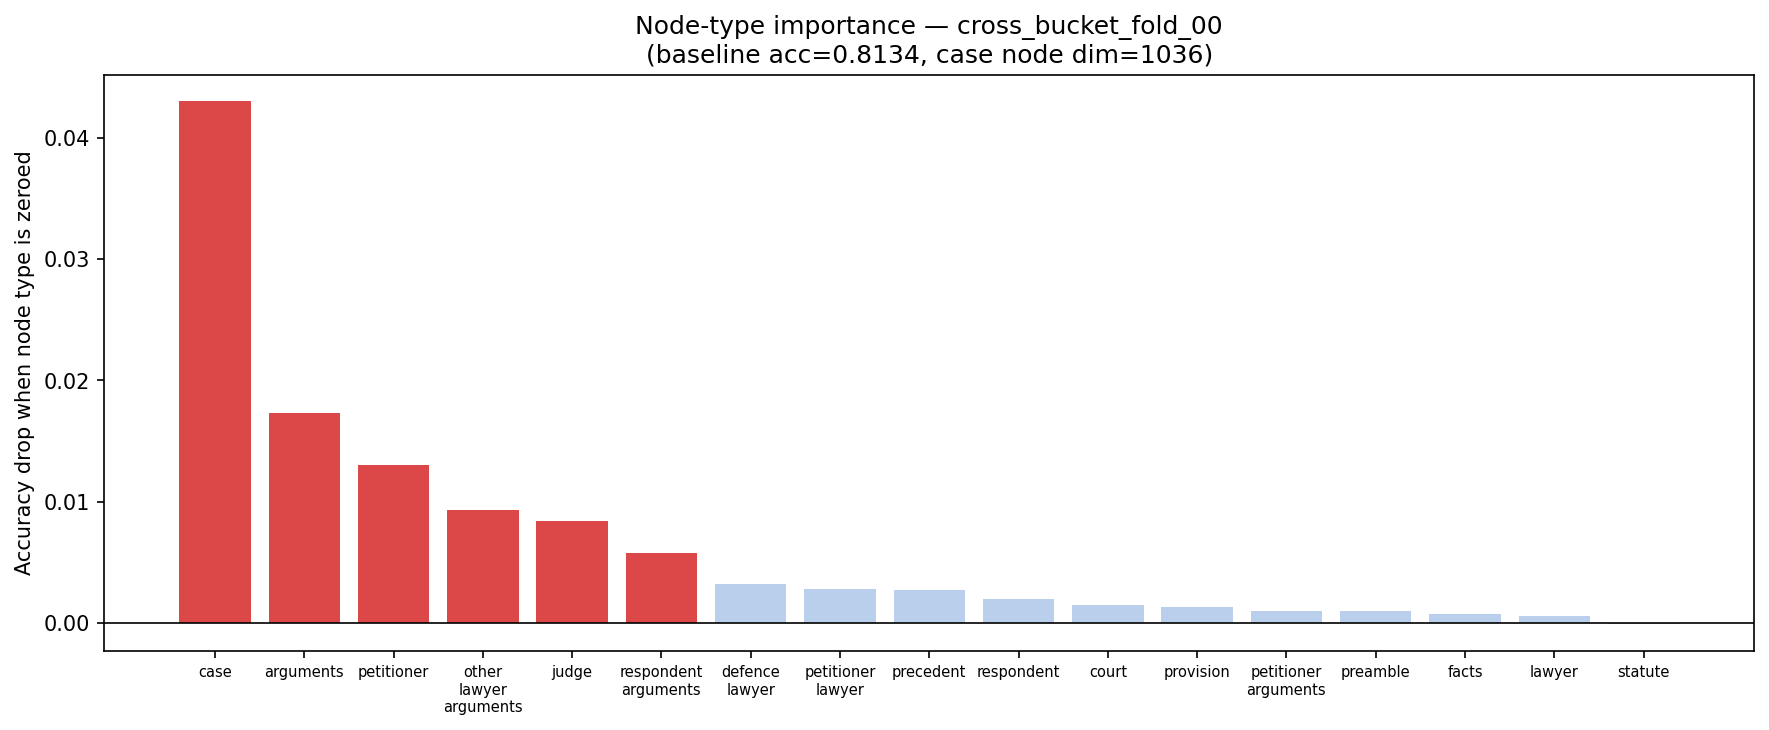
\includegraphics[width=\linewidth]{figures/explainability/node_importance.png}
    \end{column}
    \begin{column}{0.46\textwidth}
      \begin{block}{Zeroing Result}
        The \textsc{Case} node matters most, followed by the argument-bearing text stream and immediate participants such as petitioners and judges.
      \end{block}
      \begin{block}{Interpretation}
        The model is still anchored in the case representation, but it is not purely self-contained. The graph-local legal context changes the prediction materially.
      \end{block}
    \end{column}
  \end{columns}
\end{frame}

\begin{frame}{Edge Attention and Gradient Saliency}
  \scriptsize
  \begin{columns}[T]
    \begin{column}{0.38\textwidth}
      \centering
      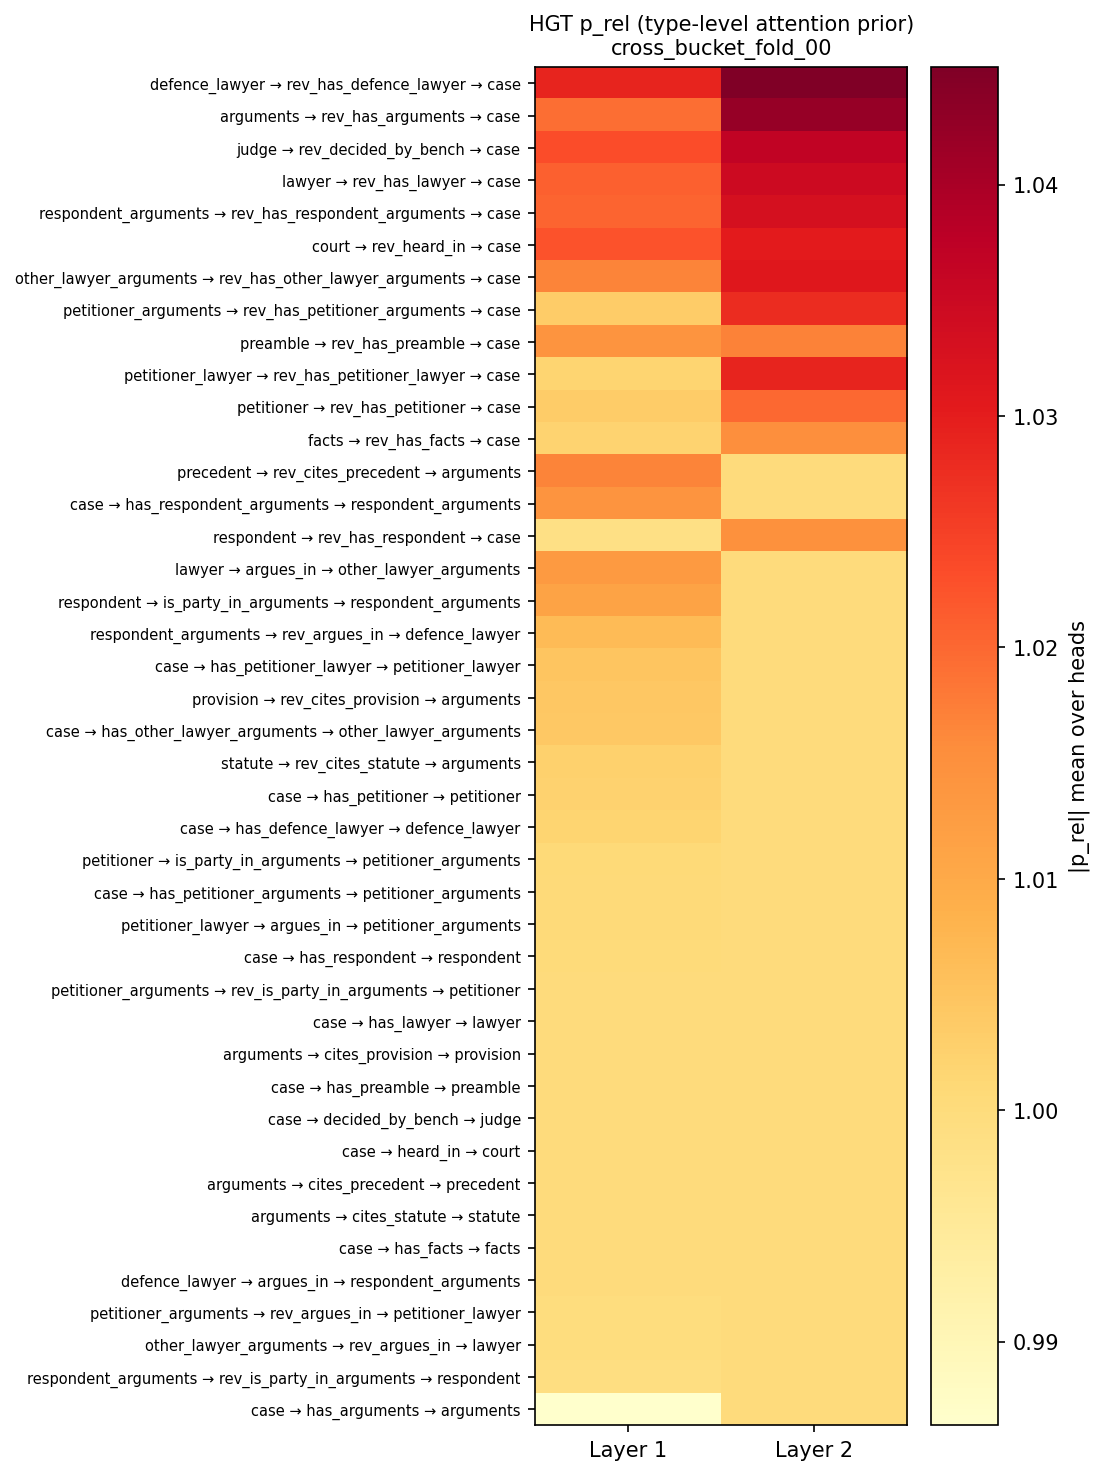
\includegraphics[width=\linewidth,height=0.66\textheight,keepaspectratio]{figures/explainability/prel_heatmap.png}
    \end{column}
    \begin{column}{0.38\textwidth}
      \centering
      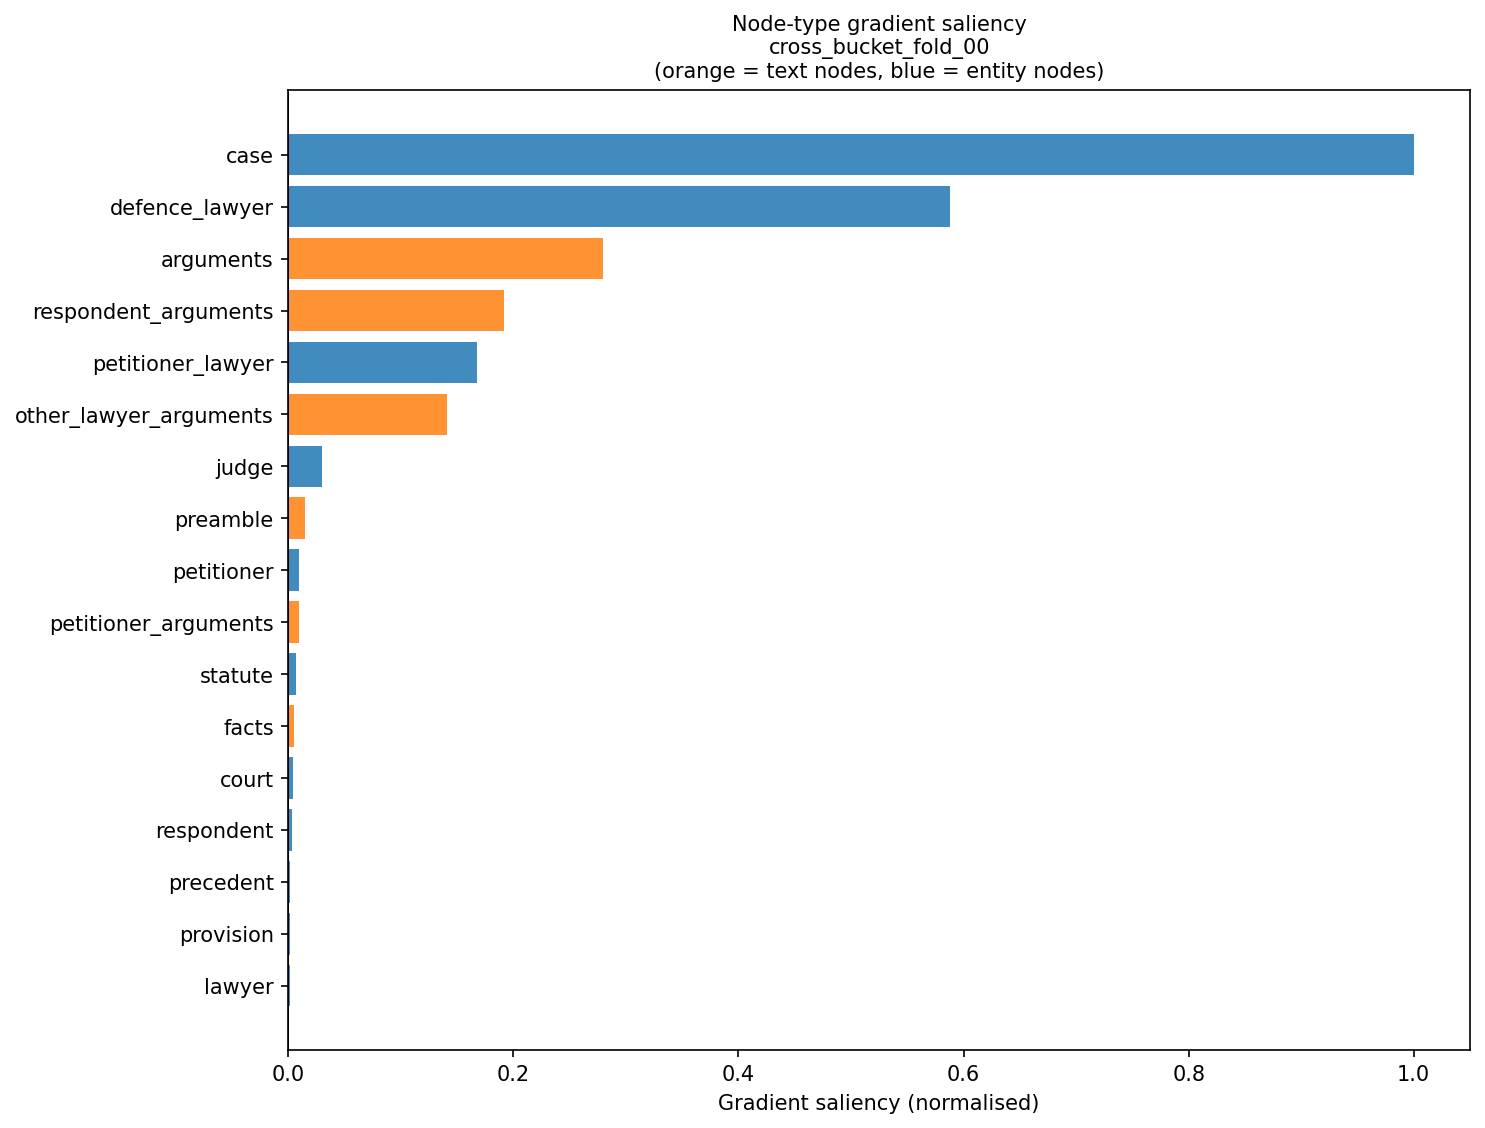
\includegraphics[width=\linewidth,height=0.66\textheight,keepaspectratio]{figures/explainability/gradient_saliency.png}
    \end{column}
    \begin{column}{0.20\textwidth}
      \begin{tightitemize}
        \item reverse edges into the case node dominate attention
        \item argument nodes dominate saliency
        \item the model operationally hinges on how arguments feed back into the case representation
      \end{tightitemize}
    \end{column}
  \end{columns}
\end{frame}

\begin{frame}{Error Decomposition: Domain and Time}
  \centering
  \begin{columns}[T]
    \begin{column}{0.48\textwidth}
      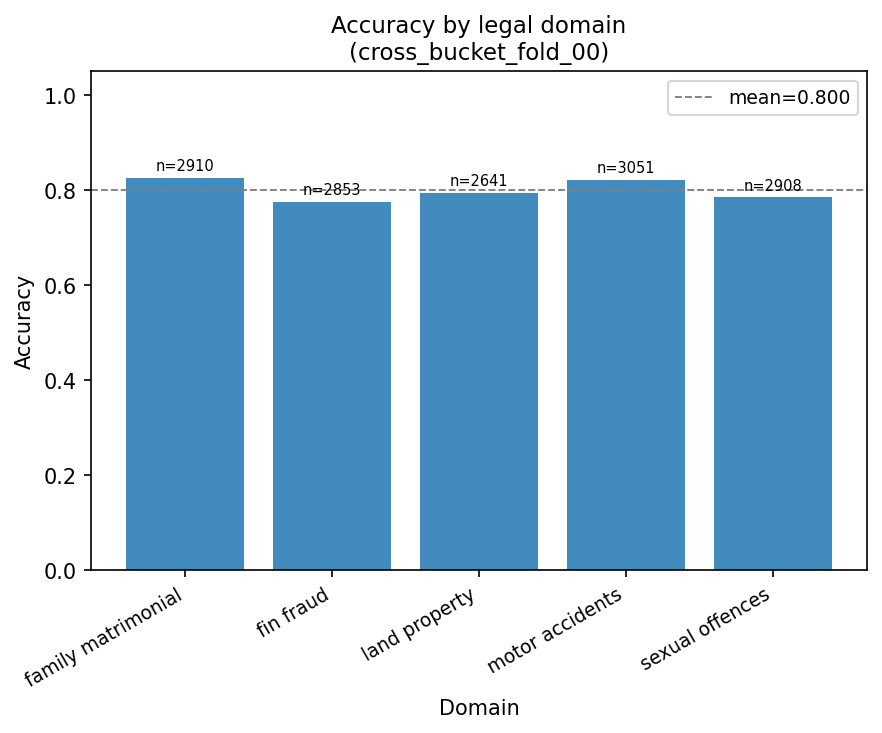
\includegraphics[width=\linewidth]{figures/explainability/error_by_domain.png}
    \end{column}
    \begin{column}{0.48\textwidth}
      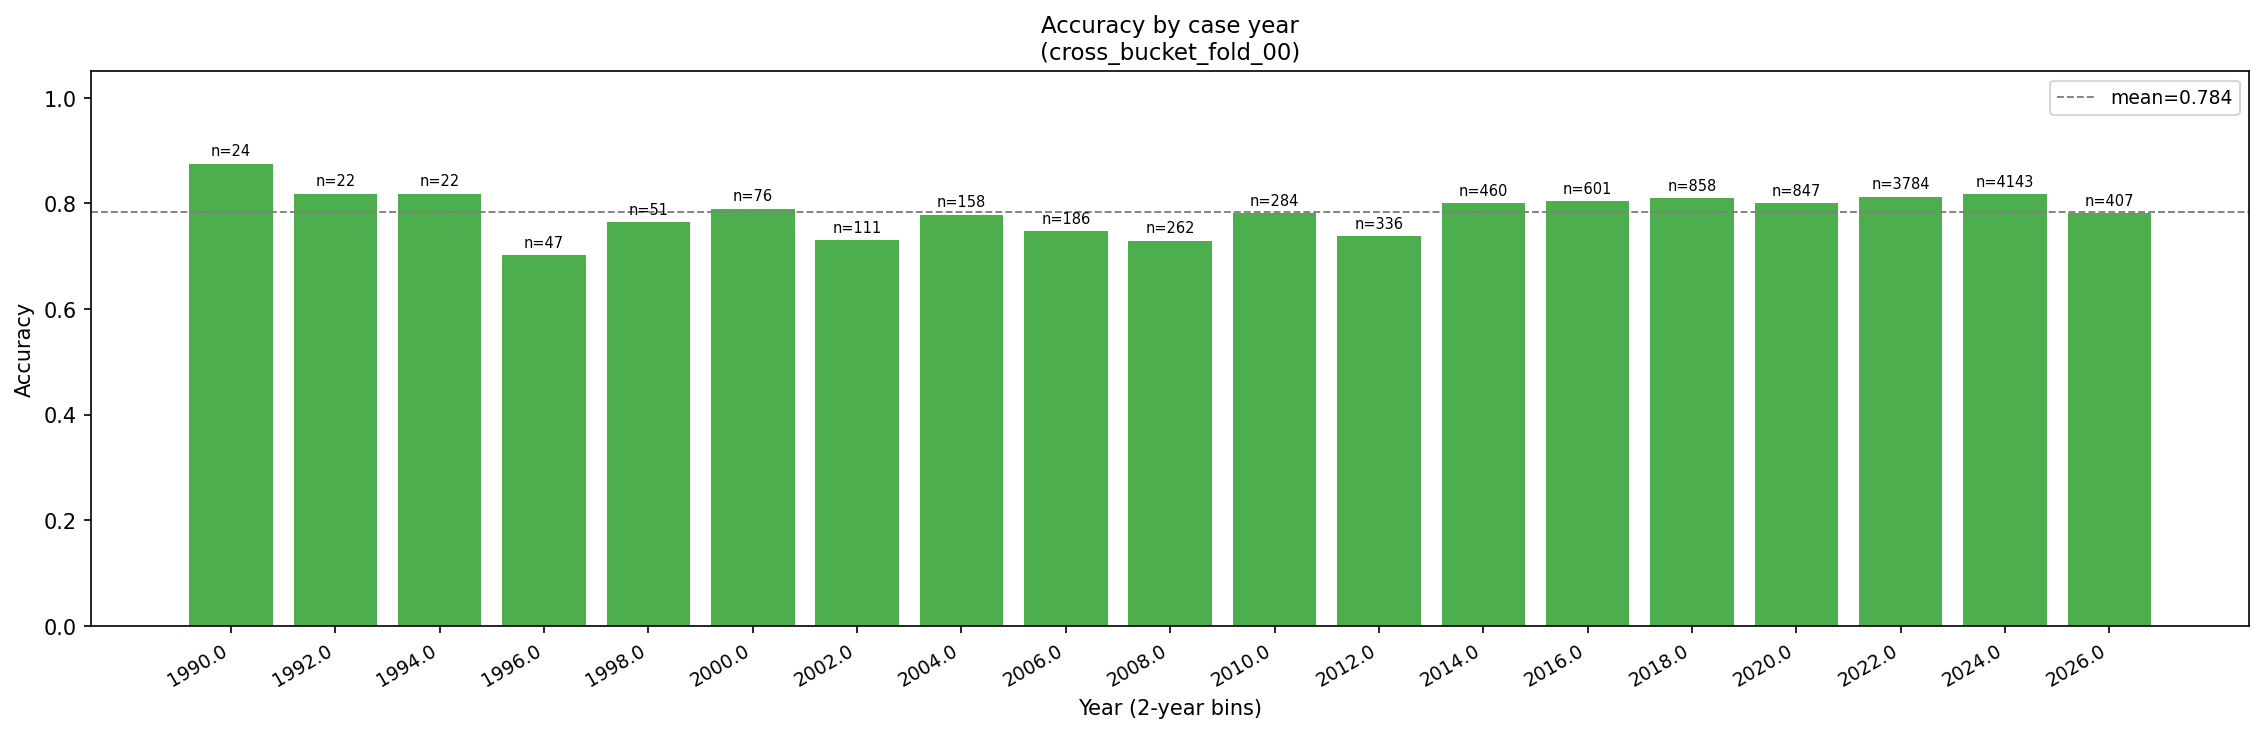
\includegraphics[width=\linewidth]{figures/explainability/error_by_year.png}
    \end{column}
  \end{columns}

  \vspace{0.6em}
  \small
  Hard domains remain hard across variants, while temporal drift is limited after very early sparse years are excluded.
\end{frame}

\begin{frame}{Error Decomposition: Structural Complexity}
  \centering
  \begin{columns}[T]
    \begin{column}{0.48\textwidth}
      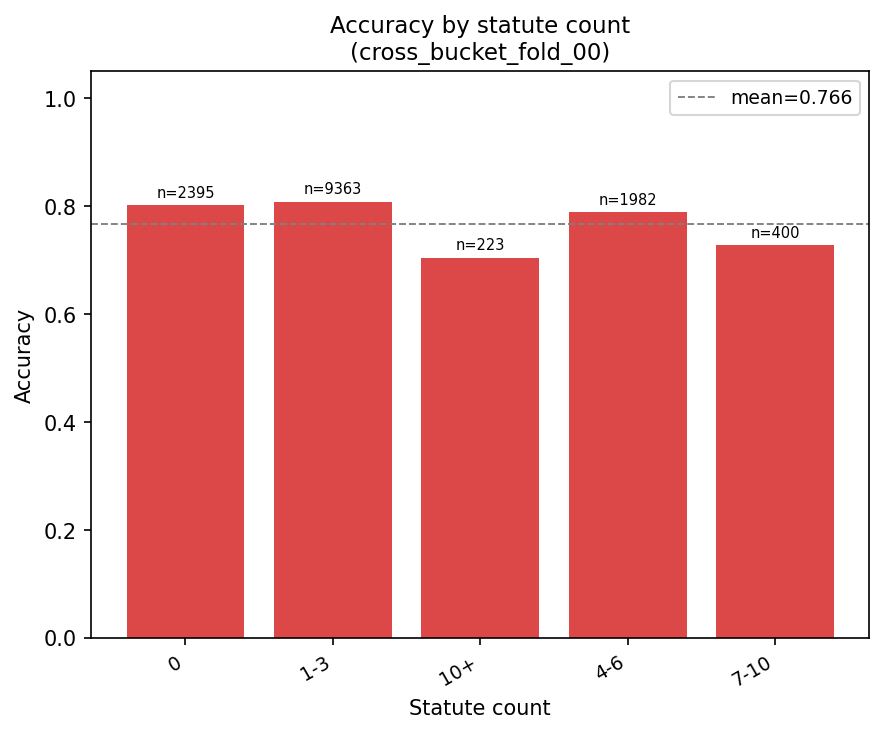
\includegraphics[width=\linewidth]{figures/explainability/error_by_statute.png}
    \end{column}
    \begin{column}{0.48\textwidth}
      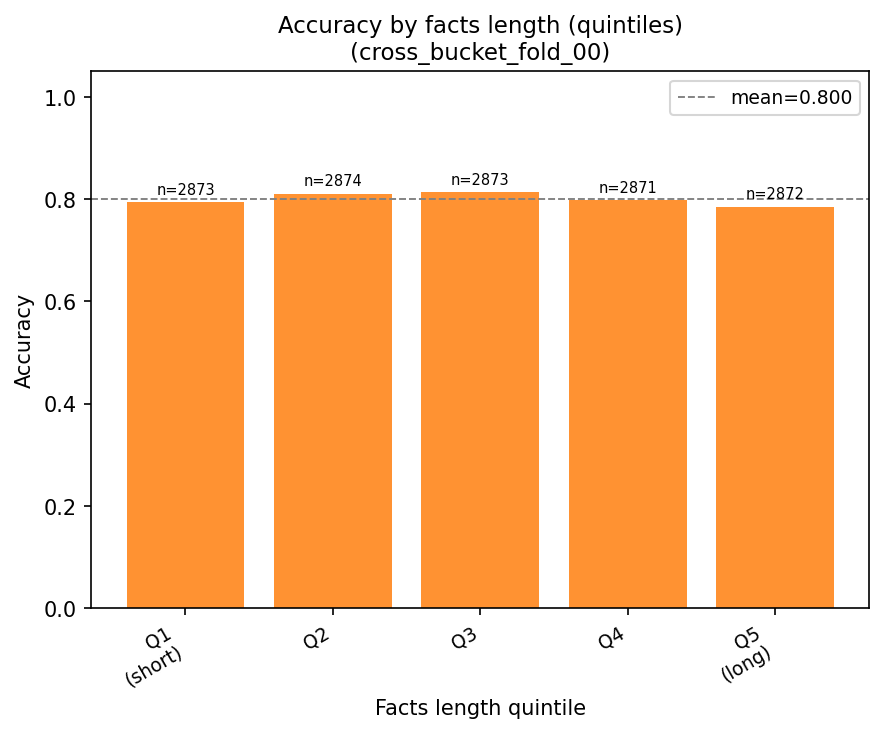
\includegraphics[width=\linewidth]{figures/explainability/error_by_facts_len.png}
    \end{column}
  \end{columns}

  \vspace{0.6em}
  \small
  Accuracy falls on \highlight{statute-dense cases} and on \highlight{the longest factual narratives}. The residual errors are about structural complexity, not about withheld names.
\end{frame}

\begin{frame}{Case-Level Explanation: A Confidently Correct Prediction}
  \scriptsize
  \begin{columns}[T,onlytextwidth]
    \begin{column}{0.44\textwidth}
      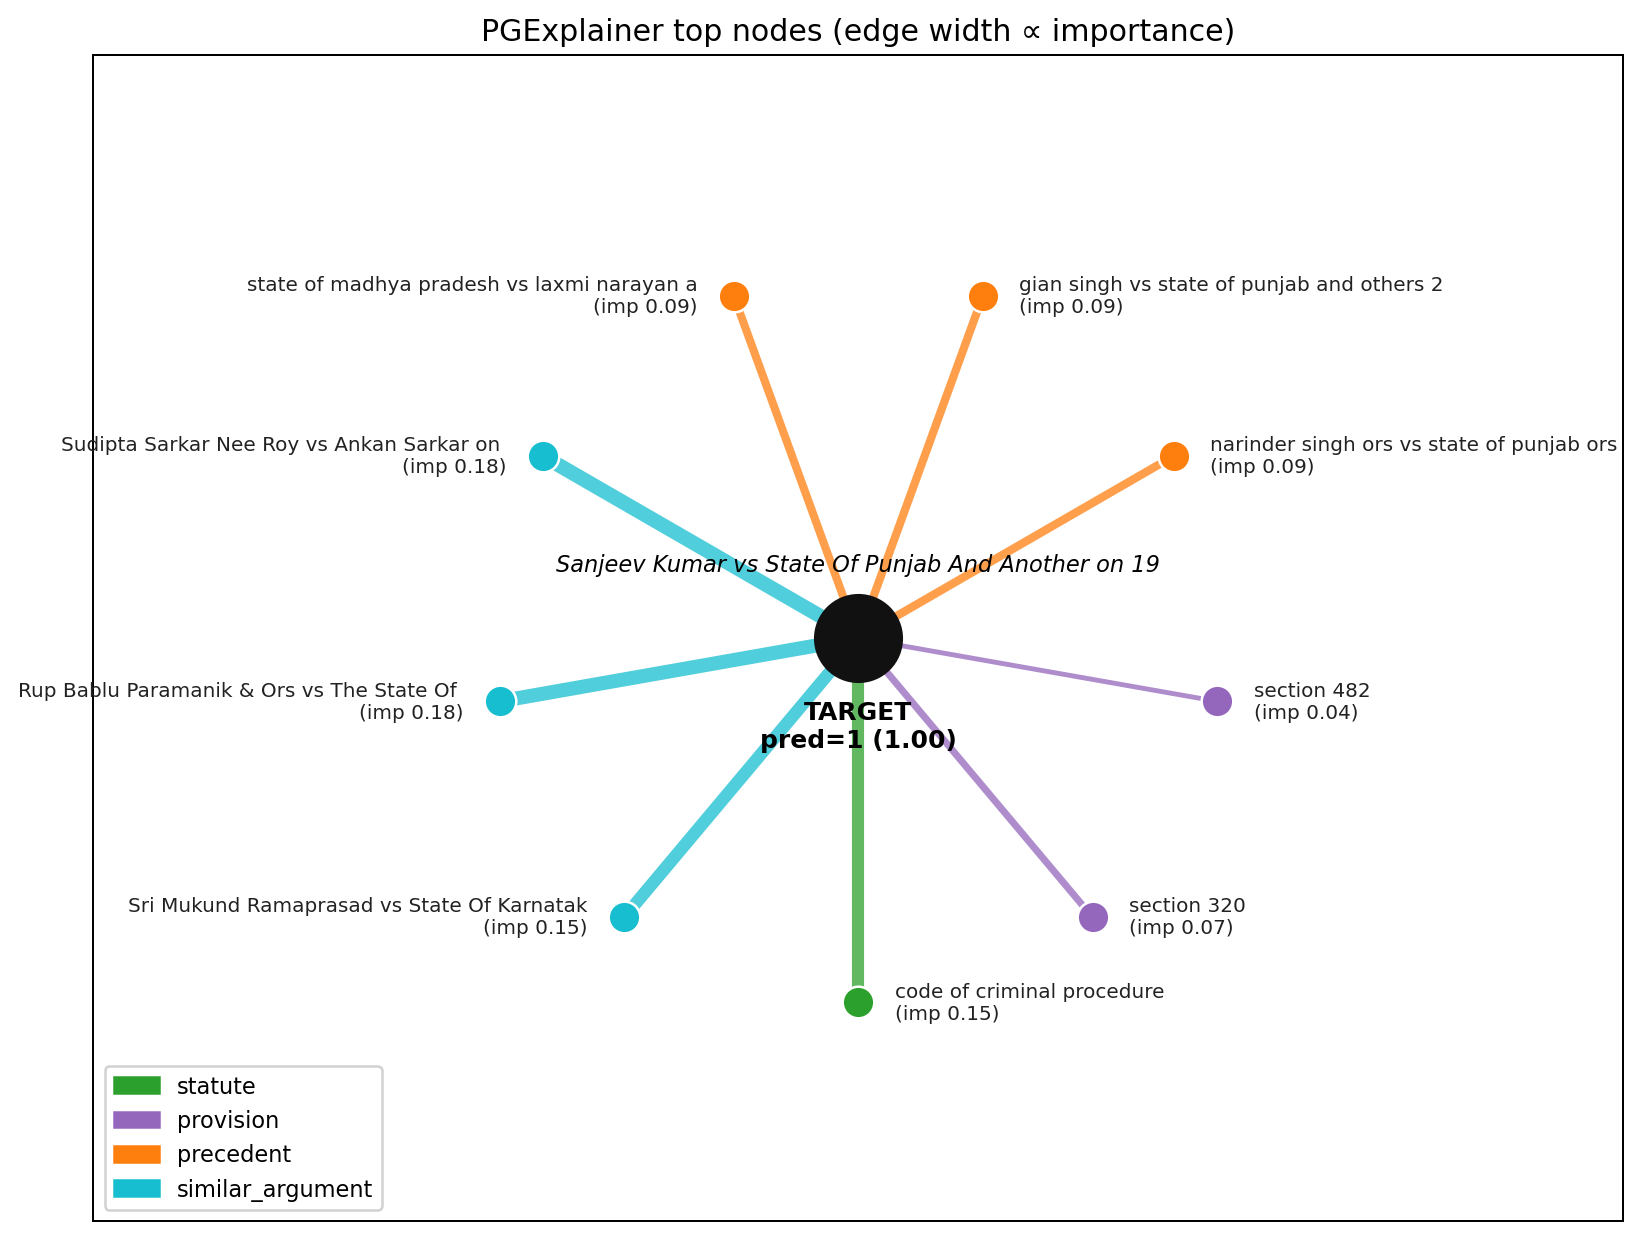
\includegraphics[width=\linewidth,height=0.58\textheight,keepaspectratio]{figures/explainability/correct_10212_panel_b_subgraph.png}
    \end{column}
    \begin{column}{0.52\textwidth}
      \begin{block}{Case 10212}
        \emph{Sanjeev Kumar vs State of Punjab} (2023)\\
        Predicted: \highlight{petitioner wins} with probability 0.9998\\
        Ground truth: \highlight{petitioner wins}
      \end{block}
      \begin{block}{Evidence the Explainer Extracts}
        \begin{tightitemize}
          \item governing statute: \textsc{CrPC}
          \item top provisions: Section~320 and Section~482 CrPC
          \item retrieved neighbours: other Punjab quash-on-compromise wins
          \item legal pattern: compromise-driven quashing under inherent High Court power
        \end{tightitemize}
      \end{block}
    \end{column}
  \end{columns}
\end{frame}

\begin{frame}{Case-Level Explanation: When Confidence and Correctness Diverge}
  \scriptsize
  \begin{columns}[T,onlytextwidth]
    \begin{column}{0.54\textwidth}
      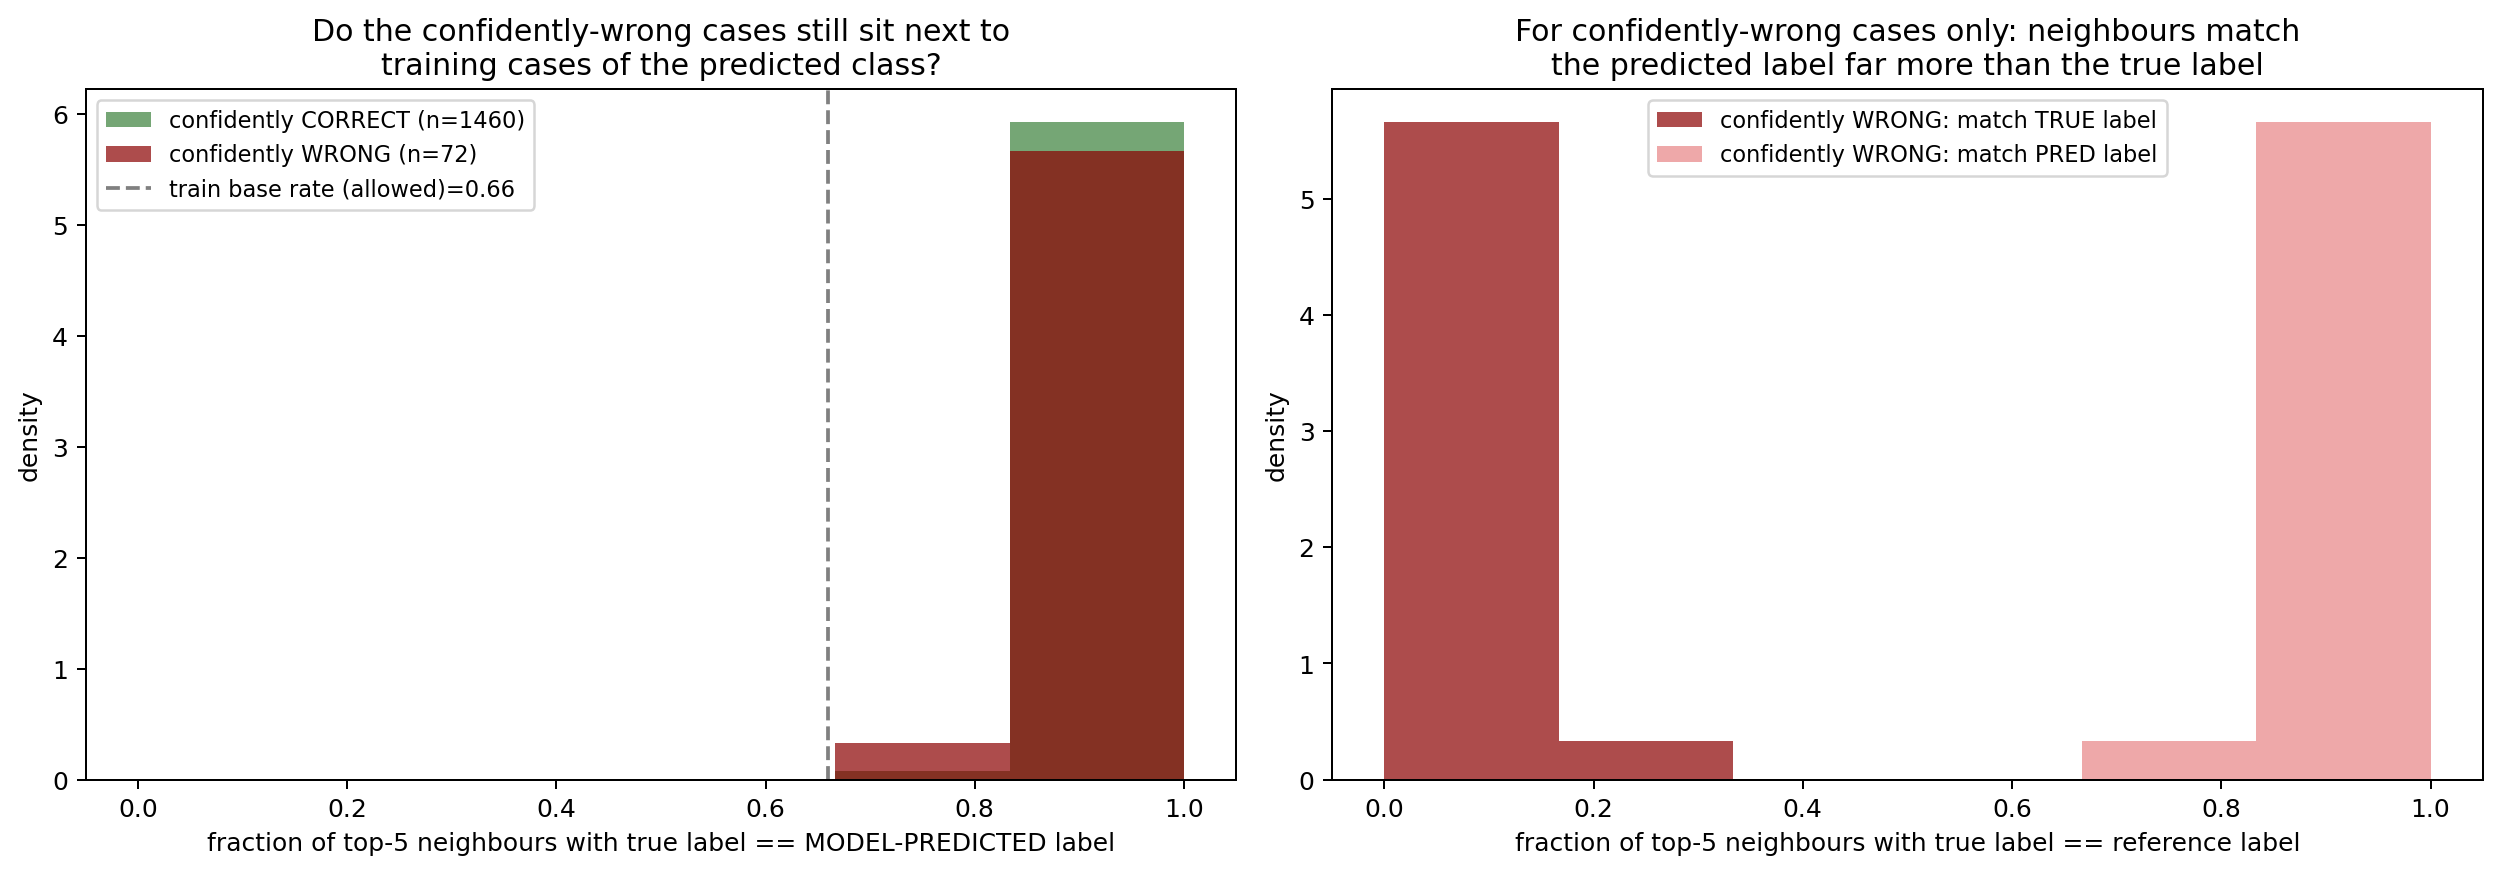
\includegraphics[width=\linewidth,height=0.62\textheight,keepaspectratio]{figures/explainability/neighbour_alignment_hist.png}
    \end{column}
    \begin{column}{0.40\textwidth}
      \begin{block}{Why This Matters}
        Among high-confidence predictions, \highlight{72 cases are confidently wrong}. Their retrieved neighbours overwhelmingly match the \emph{predicted wrong class}, which means the explanation pipeline exposes the failure instead of hiding it.
      \end{block}
      \begin{block}{Structural Signature}
        A confident error is a case placed inside the wrong outcome neighbourhood in embedding space.
      \end{block}
    \end{column}
  \end{columns}
\end{frame}

\begin{frame}{Worked Example of a Confidently Wrong Case}
  \scriptsize
  \begin{columns}[T,onlytextwidth]
    \begin{column}{0.44\textwidth}
      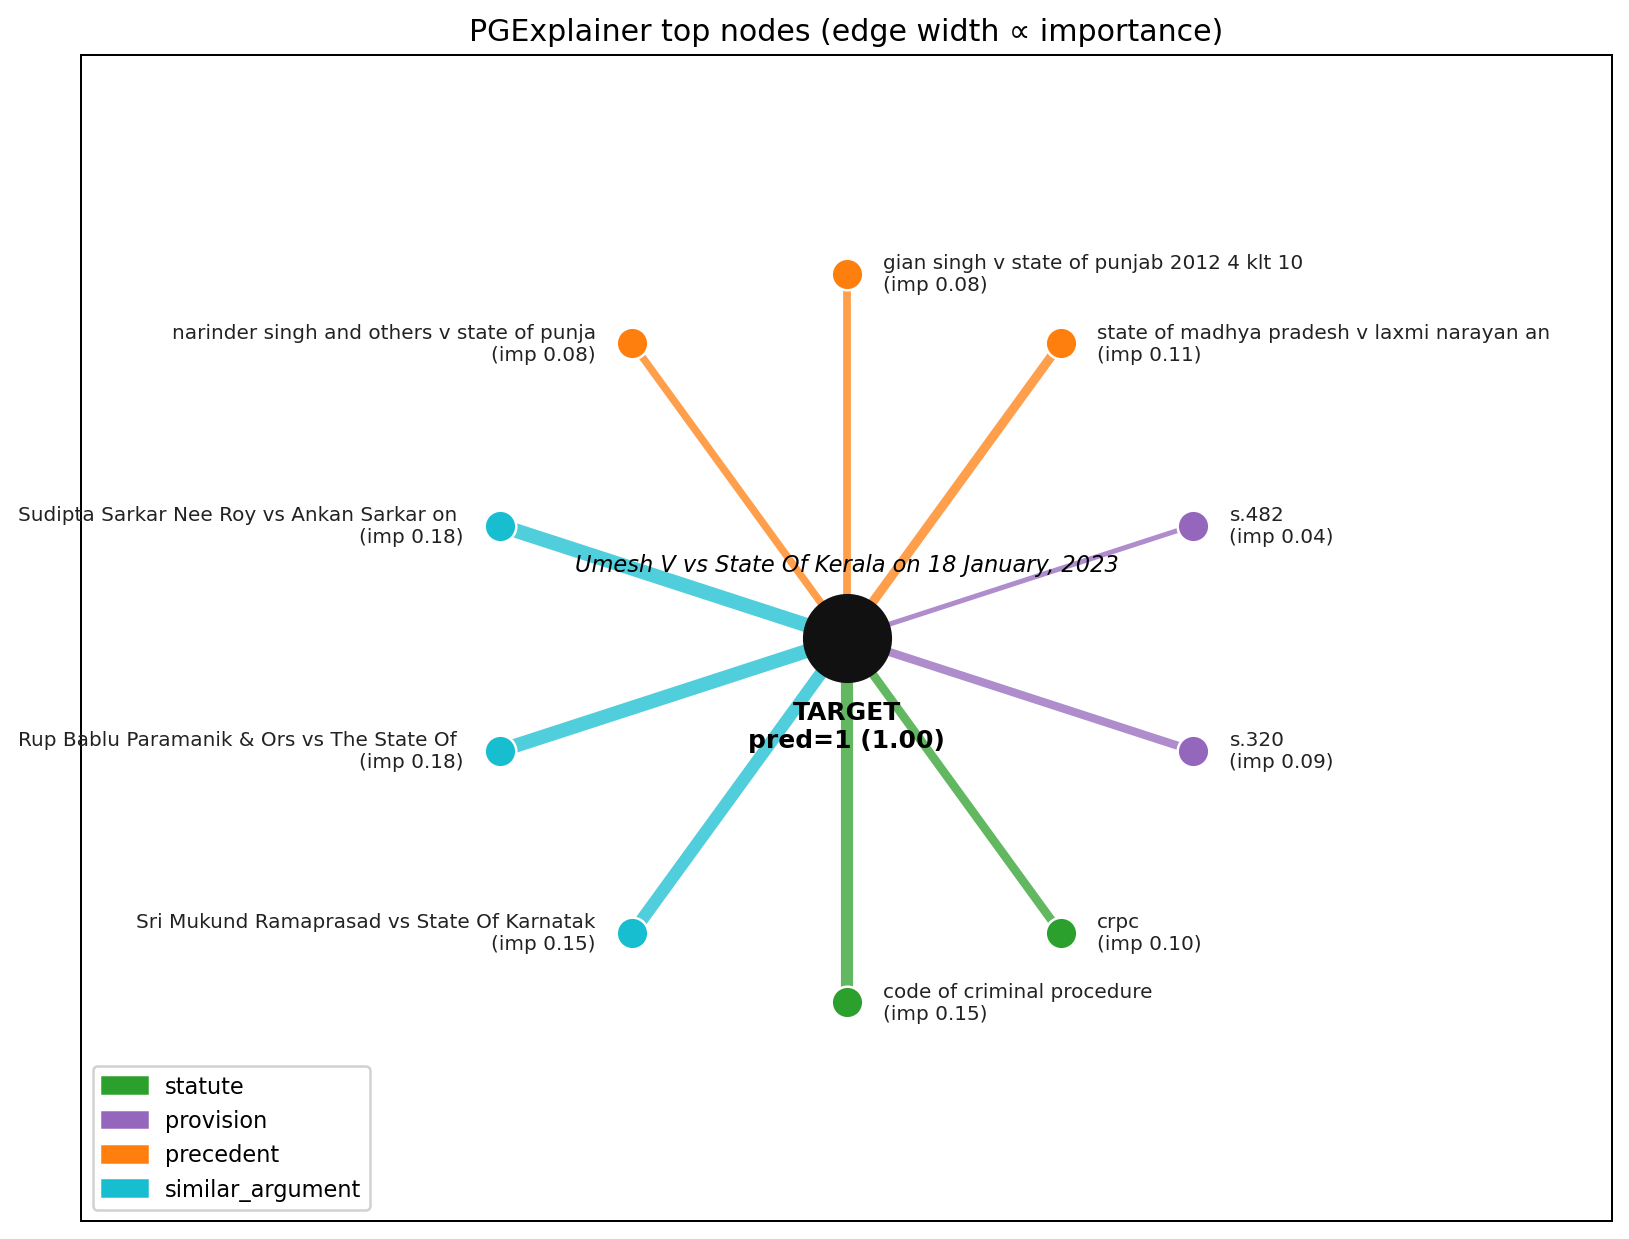
\includegraphics[width=\linewidth,height=0.58\textheight,keepaspectratio]{figures/explainability/wrong_13701_panel_b_subgraph.png}
    \end{column}
    \begin{column}{0.52\textwidth}
      \begin{block}{Case 13701}
        \emph{Umesh V vs State of Kerala} (2023)\\
        Predicted: \highlight{petitioner wins} with probability 0.9998\\
        Ground truth: \highlight{petitioner loses}
      \end{block}
      \begin{block}{Interpretation}
        The local evidence is not random noise. The target case sits in a neighbourhood of structurally similar Kerala win cases, so both prediction and retrieval reinforce the same wrong class.
      \end{block}
    \end{column}
  \end{columns}
\end{frame}

\section{Discussion and Conclusion}

\begin{frame}{Thesis at a Glance}
  \scriptsize
  \begin{columns}[T]
    \begin{column}{0.48\textwidth}
      \begin{block}{Problem}
        Indian court judgments are long, noisy, multi-hearing, and structurally heterogeneous. Naive text classification risks reading the answer from decision text or identity shortcuts.
      \end{block}
      \begin{block}{Core Idea}
        Convert judgments into a \highlight{leakage-audited heterogeneous legal graph} so the model reasons over cases, parties, arguments, statutes, provisions, precedents, courts, and judges as typed objects.
      \end{block}
    \end{column}
    \begin{column}{0.48\textwidth}
      \begin{block}{Data Scale}
        \begin{tightitemize}
          \item 5 legal domains
          \item 75{,}941 raw hearing documents
          \item 73{,}804 final merged cases
          \item 72{,}735 binary-labelled cases used in the pooled prediction task
        \end{tightitemize}
      \end{block}
      \begin{block}{Headline Result}
        Best pooled model:
        \[
        \begin{aligned}
        \metric{80.20\%} &\text{ accuracy}\\
        \metric{0.7959} &\text{ macro-F1}\\
        \metric{0.8831} &\text{ ROC-AUC}
        \end{aligned}
        \]
        On $N\!=\!14{,}363$ pooled test cases, this is $\sim$\highlight{$+6$ pts macro-F1} over no-graph logistic regression using the same BGE-M3 features.
      \end{block}
    \end{column}
  \end{columns}
\end{frame}

\begin{frame}{What the Thesis Establishes}
  \scriptsize
  \begin{block}{Main Findings}
    \begin{tightitemize}
      \item The thesis builds a \highlight{legally coherent, large-scale Indian legal corpus} from raw judgments with explicit leakage auditing.
      \item A reasoning-focused heterogeneous graph improves by $\sim$\,\highlight{$+6$ pts macro-F1} over a no-graph logistic-regression baseline using the same BGE-M3 case features.
      \item The gain decomposes into \highlight{case--section message passing}, a smaller entity-layer contribution, and optimisation/encoder refinements --- not identity memorization or direct decision leakage.
      \item The hardest remaining error mode is class-specific: the minority outcome class has lower F1, and the best pooled variant wins because it improves both classes together.
      \item The learned representation is auditable globally and locally.
      \item The pooled model transfers partially to an unseen legal domain without fine-tuning.
    \end{tightitemize}
  \end{block}
  \begin{block}{Most Defensible Claim}
    Graph-based legal prediction is most credible when it is \highlight{structurally faithful, experimentally honest, and auditable case-by-case}.
  \end{block}
\end{frame}

\begin{frame}{Limitations}
  \scriptsize
  \begin{columns}[T,onlytextwidth]
    \begin{column}{0.48\textwidth}
      \begin{block}{Data and Evaluation}
        \begin{tightitemize}
          \item Main numbers are transductive, so entity overlap at test time is partly assumed.
          \item Outcome labels are LLM-generated and therefore noisy, especially around procedural dispositions.
          \item Leakage filtering lowers risk but cannot mathematically prove zero leakage in every case.
        \end{tightitemize}
      \end{block}
    \end{column}
    \begin{column}{0.48\textwidth}
      \begin{block}{Modeling Limits}
        \begin{tightitemize}
          \item Ablation margins are often small, so some variants should be treated as a cluster rather than a strict ranking.
          \item The no-graph LR reference is currently reported from the fold-0 probing pipeline; a fully matched comparison should run that probe across all 5 folds.
          \item The pooled optimum is not the universal optimum for every legal domain.
          \item Out-of-domain transfer is meaningful but still far below in-domain performance.
        \end{tightitemize}
      \end{block}
    \end{column}
  \end{columns}
\end{frame}

\begin{frame}{Future Work}
  \begin{columns}[T]
    \begin{column}{0.48\textwidth}
      \begin{block}{Methodological Next Steps}
        \begin{tightitemize}
          \item inductive temporal and court hold-out splits
          \item multi-label or ordinal outcome targets
          \item stronger identity-leakage audits
          \item connectivity-aware and domain-adaptive modeling
        \end{tightitemize}
      \end{block}
    \end{column}
    \begin{column}{0.48\textwidth}
      \begin{block}{Practical Next Steps}
        \begin{tightitemize}
          \item expert review of case-level explanations
          \item expansion to more legal domains
          \item light-weight fine-tuning for unseen domains
          \item deployment-time uncertainty signals based on class-boundary proximity, not confidence alone
        \end{tightitemize}
      \end{block}
    \end{column}
  \end{columns}
\end{frame}

\begin{frame}[plain]
  \vfill
  \begin{center}
    {\usebeamerfont{title}\color{ThesisBlue} \Large Closing Takeaway\par}
    \vspace{1.2em}
    {\large
    This thesis argues that legal judgment prediction should be treated as a \highlight{structured legal reasoning problem}, not a flat text-classification problem.\par}
    \vspace{1.0em}
    {\large
    The contribution is not just a stronger score, but a pipeline that is \highlight{leakage-audited, graph-grounded, interpretable, and partially transferable}.}
  \end{center}
  \vfill
\end{frame}

\section{Appendix: Companion Tables}

\begin{frame}{Appendix --- Accuracy Across All Variants and Domains}
  \tiny
  \centering
  \setlength{\tabcolsep}{3pt}
  \begin{adjustbox}{max width=\textwidth}
    \begin{tabular}{lccccccc}
      \toprule
      \textbf{Model} & \textbf{Family} & \textbf{Fin.\ Fraud} & \textbf{Land/Prop.} & \textbf{Motor Acc.} & \textbf{Sexual Off.} & \textbf{Cross-bucket} & \textbf{Mean$_5$} \\
      \midrule
      \texttt{LR (no graph)}$^\dagger$          & 0.7762               & 0.7043               & 0.7280               & 0.7903               & 0.7171               & 0.7443               & 0.7432 \\
      \texttt{text\_only} (graph $-$ entities)  & 0.8205\,$\pm$\,0.007 & 0.7635\,$\pm$\,0.008 & 0.8062\,$\pm$\,0.010 & 0.8249\,$\pm$\,0.004 & 0.7732\,$\pm$\,0.006 & 0.7732\,$\pm$\,0.006 & 0.7977 \\
      \texttt{baseline} (HGT)                   & 0.8217\,$\pm$\,0.008 & 0.7683\,$\pm$\,0.009 & 0.8083\,$\pm$\,0.005 & 0.8420\,$\pm$\,0.004 & 0.7752\,$\pm$\,0.007 & 0.7811\,$\pm$\,0.006 & 0.8031 \\
      \texttt{hierarchical\_enc}                & \textbf{0.8275\,$\pm$\,0.009} & 0.7668\,$\pm$\,0.011 & 0.8029\,$\pm$\,0.010 & 0.8439\,$\pm$\,0.006 & \underline{0.7780\,$\pm$\,0.008} & 0.7811\,$\pm$\,0.003 & 0.8038 \\
      \texttt{section\_sep\_enc}                & \underline{0.8270\,$\pm$\,0.009} & \textbf{0.7717\,$\pm$\,0.012} & 0.8104\,$\pm$\,0.009 & 0.8430\,$\pm$\,0.007 & 0.7745\,$\pm$\,0.008 & \underline{0.7892\,$\pm$\,0.009} & \textbf{0.8053} \\
      \textbf{\texttt{party\_args\_lr\_decay}}  & 0.8254\,$\pm$\,0.003 & \underline{0.7709\,$\pm$\,0.011} & 0.8103\,$\pm$\,0.006 & 0.8413\,$\pm$\,0.003 & \textbf{0.7809\,$\pm$\,0.004} & \textbf{0.8020\,$\pm$\,0.004} & \underline{0.8058} \\
      \texttt{no\_names}                        & 0.8251\,$\pm$\,0.006 & 0.7702\,$\pm$\,0.011 & \underline{0.8104\,$\pm$\,0.011} & \textbf{0.8461\,$\pm$\,0.002} & 0.7743\,$\pm$\,0.010 & 0.7866\,$\pm$\,0.007 & 0.8052 \\
      \texttt{no\_cross\_case}                  & 0.8246\,$\pm$\,0.007 & 0.7688\,$\pm$\,0.013 & \textbf{0.8105\,$\pm$\,0.009} & 0.8418\,$\pm$\,0.003 & 0.7751\,$\pm$\,0.008 & 0.7837\,$\pm$\,0.005 & 0.8042 \\
      \texttt{case\_node\_minimised}            & 0.8195\,$\pm$\,0.004 & 0.7678\,$\pm$\,0.009 & 0.8011\,$\pm$\,0.008 & \underline{0.8423\,$\pm$\,0.011} & 0.7750\,$\pm$\,0.006 & 0.7755\,$\pm$\,0.003 & 0.8011 \\
      \bottomrule
    \end{tabular}
  \end{adjustbox}

  \vspace{0.5em}
  \scriptsize Mean $\pm$ std over 5 folds for HGT variants. \textbf{Bold} = best per column; \underline{underline} = second best. \textbf{Mean$_5$} = unweighted average across the five per-domain columns. In this single-label binary setting, micro-F1 is numerically identical to accuracy, so a separate micro-F1 table is omitted.\\
  $^\dagger$\,\texttt{LR (no graph)}: logistic regression on BGE-M3 case-text embedding $+$ 12 scalar case features --- no graph, no message passing. Reported on fold 0.
\end{frame}

\begin{frame}{Appendix --- ROC-AUC Across All Variants and Domains}
  \tiny
  \centering
  \setlength{\tabcolsep}{3pt}
  \begin{adjustbox}{max width=\textwidth}
    \begin{tabular}{lccccccc}
      \toprule
      \textbf{Model} & \textbf{Family} & \textbf{Fin.\ Fraud} & \textbf{Land/Prop.} & \textbf{Motor Acc.} & \textbf{Sexual Off.} & \textbf{Cross-bucket} & \textbf{Mean$_5$} \\
      \midrule
      \texttt{text\_only}                       & 0.8944\,$\pm$\,0.005 & 0.8407\,$\pm$\,0.005 & 0.8638\,$\pm$\,0.004 & 0.8880\,$\pm$\,0.004 & \textbf{0.8495\,$\pm$\,0.004} & 0.8561\,$\pm$\,0.007 & 0.8673 \\
      \texttt{baseline} (HGT)                   & 0.8923\,$\pm$\,0.008 & 0.8406\,$\pm$\,0.006 & 0.8645\,$\pm$\,0.006 & 0.9010\,$\pm$\,0.005 & 0.8442\,$\pm$\,0.006 & 0.8674\,$\pm$\,0.002 & 0.8685 \\
      \texttt{hierarchical\_enc}                & \underline{0.8963\,$\pm$\,0.009} & 0.8403\,$\pm$\,0.009 & \textbf{0.8676\,$\pm$\,0.007} & \underline{0.9037\,$\pm$\,0.007} & \underline{0.8462\,$\pm$\,0.007} & 0.8655\,$\pm$\,0.003 & \underline{0.8708} \\
      \texttt{section\_sep\_enc}                & \textbf{0.8968\,$\pm$\,0.006} & \textbf{0.8416\,$\pm$\,0.011} & \underline{0.8676\,$\pm$\,0.005} & \textbf{0.9044\,$\pm$\,0.004} & 0.8441\,$\pm$\,0.006 & \underline{0.8712\,$\pm$\,0.008} & \textbf{0.8709} \\
      \textbf{\texttt{party\_args\_lr\_decay}}  & 0.8940\,$\pm$\,0.006 & 0.8373\,$\pm$\,0.008 & 0.8625\,$\pm$\,0.007 & 0.9024\,$\pm$\,0.006 & 0.8436\,$\pm$\,0.006 & \textbf{0.8831\,$\pm$\,0.002} & 0.8680 \\
      \texttt{no\_names}                        & 0.8959\,$\pm$\,0.003 & \underline{0.8416\,$\pm$\,0.005} & 0.8640\,$\pm$\,0.009 & 0.9022\,$\pm$\,0.006 & 0.8441\,$\pm$\,0.007 & 0.8665\,$\pm$\,0.006 & 0.8695 \\
      \texttt{no\_cross\_case}                  & 0.8951\,$\pm$\,0.007 & 0.8410\,$\pm$\,0.008 & 0.8637\,$\pm$\,0.003 & 0.9031\,$\pm$\,0.002 & 0.8421\,$\pm$\,0.005 & 0.8658\,$\pm$\,0.002 & 0.8690 \\
      \texttt{case\_node\_minimised}            & 0.8881\,$\pm$\,0.008 & 0.8332\,$\pm$\,0.008 & 0.8552\,$\pm$\,0.009 & 0.9020\,$\pm$\,0.005 & 0.8320\,$\pm$\,0.010 & 0.8560\,$\pm$\,0.001 & 0.8621 \\
      \bottomrule
    \end{tabular}
  \end{adjustbox}

  \vspace{0.5em}
  \scriptsize Mean $\pm$ std over 5 folds. \textbf{Bold} = best per column; \underline{underline} = second best. ROC-AUC tells a slightly different story than macro-F1: the encoder variants (\texttt{section\_sep\_enc}, \texttt{hierarchical\_enc}) lead on per-domain ranking quality, while \texttt{party\_args\_lr\_decay} dominates on the pooled task.
\end{frame}

\end{document}
